\chapter{Resultados}

\noindent En este último capítulo se analizan los resultados el experimento en ambos ambientes. 

Para cada proceso se registró el tiempo total de ejecución, el tiempo de escritura, el tiempo entre el envío del comando y el tiempo de inicio de la ejecución, el porcentaje de ejecuciones completadas de manera exitosa y cómo estas cantidades escalan al cambiar de ambiente y de número de datos a procesar.

Durante esta investigación buscamos conocer la rapidez con la que cada herramienta ejecuta cada tarea pero también cómo cambia esta relación cuando modificamos el número de datos o al cambiar el ambiente de ejecución y así tener una idea de su capacidad de escalamiento. Por otro lado, buscamos ver la consistencia del tiempo de ejecución de los procesos y también conocer qué tan robusto es cada \textit{framework} para determinar si uno es más confiable que el otro para completar las tareas. Por tal motivo, las secciones \ref{section:resultados-ambiente-local} y \ref{section:resultados-ambiente-local} se dividen en una sección que analiza los resultados de cada muestra de forma independiente y concluyen con una sección que aborda el cambio del comportamiento de cada proceso a través de las diferentes muestras.

En la primera sección, nos centraremos en las siguientes características y capacidades de cada \textit{framework} y después se hará una conclusión general para cada muestra de datos. A continuación se listan los rubros que se evaluarán y en qué consistirá el análisis para determinar el mejor desempeño de una herramienta frente a la otra.

\begin{itemize}
	
	\item \textbf{Robustez} Analizar qué tan resistentes a fallos son los procesos y su confiabilidad para terminar las tareas asignadas. Las principal métrica para evaluar esto será el porcentaje de ejecuciones completadas exitosamente en cada proceso.
	
	\item \textbf{Variación} Medir la variación del tiempo de ejecución de cada proceso en cada \textit{framework} y establecer cuál de los dos es más consistente en el tiempo de ejecución. Para este análisis se utilizará la desviación estándar de el tiempo de duración y el coeficiente de variación como métricas principales.
	
	\item \textbf{Inicio de la ejecución} Comparar el tiempo que le toma a cada proceso ejecutar la primera línea de código. Esto dará una idea de qué tanto tiempo le toma a cada herramienta la asignación de recursos y configuraciones previas a la ejecución del código. La principal métrica para comparar será el tiempo registrado entre la ejecución del comando que inicia el proceso y la primera acción ejecutada dentro del proceso.
	
	\item \textbf{Escritura} Determinar cuál \textit{framework} es más rápido para escribir el resultado a cada destino. Se analizarán de forma separada los procesos que tienen como destino final una base de datos \textit{MySQL} y los que escriben a archivos \texttt{parquet} como destino final. La principal métrica será el tiempo de escritura registrado por cada proceso. Los procesos que escriben a archivos \texttt{parquet} son: \texttt{demoras\_aeropuerto\_destino}, \texttt{demoras\_aerolinea} y \texttt{demoras\_ruta\_aeropuerto}, mientras que los que escriben a \textit{MySQL} son: \texttt{demoras\_aeropuerto\_origen}, \texttt{demoras\_ruta\_mktid}, \texttt{flota} y \texttt{dijkstra}, aunque en caso del último proceso, el resultado escrito raramente es mayor a 5 registros. Por último, el proceso \texttt{elimina\_nulos} imprime su resultado en consola y no será considerado para el análisis de tiempo de escritura.
	
	\item \textbf{Capacidad de cómputo} Establecer qué herramienta tiene un tiempo menor de procesamiento de los datos. El tiempo de cómputo engloba el tiempo de lectura de la fuente de datos, el tiempo de cálculo de resultados y la transferencia de datos necesaria. Este tiempo no incluye el tiempo transcurrido para las tareas de escritura o el tiempo de inicio de la ejecución. La principal métrica será el tiempo total transcurrido, quitando el tiempo de escritura.
	
	\item \textbf{Duración} Contrastar el desempeño de una herramienta frente a la otra en el tiempo total de ejecución de cada proceso. La métrica para comparar los \textit{frameworks} será el tiempo de ejecución registrado en cada proceso y los ratios calculados de la siguiente manera: $\frac{\texttt{tiempo\_de\_ejecucion\_dask}}{\texttt{tiempo\_de\_ejecucion\_spark}}$ y $\frac{\texttt{tiempo\_de\_ejecucion\_spark}}{\texttt{tiempo\_de\_ejecucion\_dask}}$.
\end{itemize}

En la segunda sección, el énfasis será en el tiempo de escritura de acuerdo a las diferentes muestras y en el tiempo de ejecución total de cada proceso.

\newpage

\section{Ambiente local}
\label{section:resultados-ambiente-local}

Para empezar revisaremos los resultados de cada \textit{framework} en los distintos procesos y a través de las diferentes muestras de datos al ejecutarlos en el ambiente local. Después de una revisión individual de cada muestra de datos vamos a pasar a un análisis global en el que analizaremos la capacidad de escalamiento de la herramienta en una computadora local.

\subsection{Ejecución local con 10,000 registros}

Las conclusiones más relevantes sobre esta muestra de datos son las siguientes:

\begin{center}
\begin{figure}
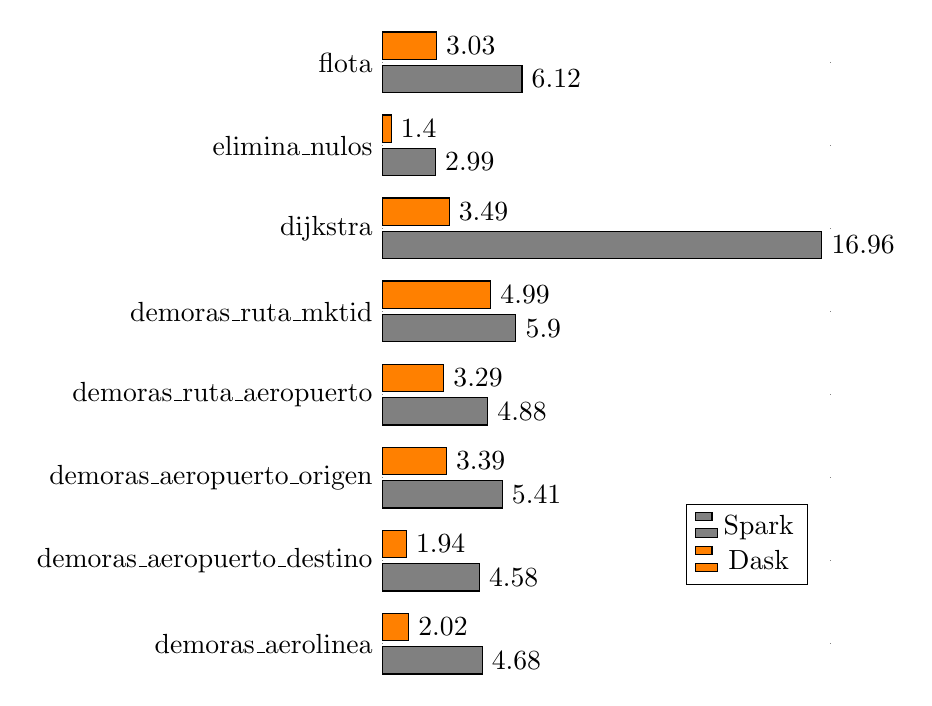
\begin{tikzpicture}
  \begin{axis}[
    xbar,
    y axis line style = { opacity = 0 },
    axis x line       = none,
    y                 = 30,
    x                 = 10,
    legend style={at={(0.95,0.25)}},
    clip              = false,
    tickwidth         = 0.1pt,
    ytick             = data,
    enlarge y limits  = 0.02,
    enlarge x limits  = 0.02,
    symbolic y coords = {demoras\_aerolinea, demoras\_aeropuerto\_destino, demoras\_aeropuerto\_origen, demoras\_ruta\_aeropuerto, demoras\_ruta\_mktid, dijkstra, elimina\_nulos, flota},
    nodes near coords,
  ]
  
  \addplot[fill=gray] coordinates { (4.678,demoras\_aerolinea)
  						(4.578,demoras\_aeropuerto\_destino)
  						(5.406,demoras\_aeropuerto\_origen)
  						(4.881,demoras\_ruta\_aeropuerto)
  						(5.901,demoras\_ruta\_mktid)
  						(16.957,dijkstra)
  						(2.993,elimina\_nulos)
  						(6.12,flota)};  
  
  \addplot[fill=orange] coordinates { (2.024,demoras\_aerolinea)
  						(1.939,demoras\_aeropuerto\_destino)
  						(3.386,demoras\_aeropuerto\_origen)
  						(3.291,demoras\_ruta\_aeropuerto)
  						(4.991,demoras\_ruta\_mktid)
  						(3.488,dijkstra)
  						(1.395,elimina\_nulos)
  						(3.029,flota)};
                         
  \legend{Spark, Dask}
  \end{axis}
\end{tikzpicture}
\caption{Duración de los procesos con 10,000 registros}
\label{barras:duracion10K}
\end{figure}
\end{center}


\begin{itemize}
	
	\item \textbf{Robustez} Con la muestra de datos más pequeña, ambos \textit{frameworks} lograron completar todos los procesos sin fallas, por lo que su estabilidad es comparable.
	
	\item \textbf{Variación} De acuerdo a los resultados expuestos en la tabla \ref{table:duracion10K}, en la mayoría de los procesos \textit{Dask} registró un coeficiente de variación mayor que \textit{Spark}, no obstante, hay que considerar que sus tiempos de ejecución fueron menores y casi nunca pasaron de 5 segundos de duración, por lo que un coeficiente de variación más grande es razonable. La única excepción a lo anterior fue el proceso \texttt{dijkstra} en el que \textit{Spark} tuvo mayor variación a pesar de tener mayor tiempo de ejecución promedio y en el que ambos \textit{frameworks} registraron la mayor variación debido en gran parte a que este proceso calcula una ruta aleatoria en cada ejecución. Además, es importante notar que la mayoría de los coeficientes de variación se mantuvieron por debajo de 0.03 con la excepción de \texttt{dijsktra} y los procesos \texttt{demoras\_ruta\_mktid}, \texttt{demoras\_ruta\_aeropuerto} y \texttt{flota} de \textit{Dask}, de los cuales dos tuvieron un coeficiente mayor a 0.4.
	
	\item \textbf{Inicio de la ejecución} Los resultados registrados en la tabla \ref{table:otros10K} muestran que una de las diferencias más evidentes entre ambos \textit{frameworks} es el tiempo que tardan en iniciar la ejecución. En el caso de \textit{Spark} este es de alrededor de un segundo, mientras que \textit{Dask} registró un promedio menor a una centésima de segundo en casi todos los casos (con la excepción de \texttt{dijkstra} que es cercano a medio segundo). Es importante notar que el tiempo de inicio de la ejecución fue calculado de forma independiente al tiempo de ejecución por lo que no está incluido dentro del mismo.
	
	\item \textbf{Escritura} \textit{Dask} registró un tiempo mucho menor en la escritura a archivos \texttt{parquet} que \textit{Spark} en todos los casos. La diferencia fue de poco menos de un segundo en los tres procesos que tienen como destino final este tipo de archivo. Por otro lado, cuando el destino de escritura es una base de datos \textit{MySQL}, \textit{Dask} también registró un mejor desempeño aunque la diferencia no es tan evidente como en el caso de archivos \texttt{parquet} ya que es de tan solo unas décimas de segundo. Esta información está expuesta en la tabla \ref{table:write10K}.
	
	\item \textbf{Capacidad de cómputo} La evidencia presentada en la tabla \ref{table:otros10K} permite ver que durante estas ejecuciones, \textit{Dask} registró un tiempo de  cómputo menor en todos los procesos, con una diferencia especialmente evidente en el proceso \texttt{dijkstra} en el que \textit{Spark} fue casi 5 veces más tardado, lo cual sucede debido a que el algoritmo es iterativo y \textit{Dask} tiene una mayor facilidad para utilizar los resultados previos ya que el resultado de cada iteración es un \textit{DataFrame} de \textit{Pandas} almacenado en memoria y \textit{Spark}, por el contrario, tiene como comportamiento predeterminado descartar la información de la ejecución anterior y volver a ejecutar todo el proceso, lo que obliga a utilizar la función \texttt{checkpoint} que escribe los resultados intermedios a disco, lo que puede resultar costoso. Respecto a los otros procesos, a excepción de \texttt{demoras\_ruta\_aeropuerto} y \texttt{demoras\_ruta\_mktid} que involucran la creación de una nueva llave y donde la diferencia en los tiempo de ejecución fue menor a décimas de segundo, \textit{Spark} registró tiempos de casi el doble que los registrados por \textit{Dask}.
	
	\item \textbf{Duración} Al considerar el tiempo de ejecución total promedio (resumido en el gráfico \ref{barras:duracion10K}), podemos ver que \textit{Dask} también tuvo un mejor desempeño en todos los procesos, especialmente en el proceso \texttt{dijkstra} que fue más de 5 veces más rápido en \textit{Dask}. Por otra parte, los procesos \texttt{demoras\_aerolinea}, \texttt{demoras\_aeropuerto\_destino} y \texttt{demoras\_aeropuerto\_origen} que involucran agregaciones como promedios, obtención del máximo y mínimo y conteos utilizando múltiples llaves para agrupar, tuvieron un tiempo de ejecución al menos 1.5 veces mayor en \textit{Spark} con mayor diferencia en los procesos que tienen \texttt{parquet} como destino. Adicionalmente, los procesos que realizan tareas de preparación de datos como los procesos \texttt{elimina\_nulos} y \texttt{flota} (cuyas tareas son borrado de registros con nulos y eliminación de duplicados respectivamente) también tuvieron un tiempo de ejecución al menos dos veces mayor en \textit{Spark}. Por último, los procesos que involucran agregaciones como promedio y desviación estándar usando una llave nueva generada a partir de columnas existentes (\texttt{demoras\_ruta\_mktid} y \texttt{demoras\_ruta\_aeropuerto}) tuvieron la menor diferencia de tiempo, siendo entre 1 y 1.5 veces mayor en \textit{Spark} que en \textit{Dask}.  
	
\end{itemize}


\begin{table}
    \centering
    \resizebox{\textwidth}{!}{
    \begin{tabular}{|l|c c c c c c c|}
    \hline
        \multicolumn{1}{|p{2.2cm}|}{\centering \textbf{proceso}} & \multicolumn{1}{p{2.2cm}}{\centering \textbf{framework}} & \multicolumn{1}{p{2.2cm}}{\centering \textbf{número de ejecuciones}} & \multicolumn{1}{p{2.2cm}}{\centering \textbf{duración promedio}} & \multicolumn{1}{p{2.2cm}}{\centering \textbf{desviación estándar}} & \multicolumn{1}{p{2.5cm}}{\centering \textbf{coeficiente de variación}} & \multicolumn{1}{p{2.2cm}}{\centering \textbf{$\frac{\texttt{dask}}{\texttt{spark}}$ (duración)}} & \multicolumn{1}{p{2.2cm}|}{\centering \textbf{$\frac{\texttt{spark}}{\texttt{dask}}$ (duración)}} \\ \hline
        demoras\_aerolinea & dask & 100 & 2.024 & 0.048 & 0.024 & 0.433 & 2.311 \\ % \hline
        demoras\_aerolinea & spark & 100 & 4.678 & 0.065 & 0.014 & 0.433 & 2.311 \\ % \hline
        demoras\_aeropuerto\_destino & dask & 100 & 1.939 & 0.043 & 0.022 & 0.424 & 2.361 \\ % \hline
        demoras\_aeropuerto\_destino & spark & 100 & 4.578 & 0.064 & 0.014 & 0.424 & 2.361 \\ % \hline
        demoras\_aeropuerto\_origen & dask & 100 & 3.386 & 0.095 & 0.028 & 0.626 & 1.597 \\ % \hline
        demoras\_aeropuerto\_origen & spark & 100 & 5.406 & 0.132 & 0.024 & 0.626 & 1.597 \\ % \hline
        demoras\_ruta\_aeropuerto & dask & 100 & 3.291 & 1.688 & 0.513 & 0.674 & 1.483 \\ % \hline
        demoras\_ruta\_aeropuerto & spark & 100 & 4.881 & 0.091 & 0.019 & 0.674 & 1.483 \\ % \hline
        demoras\_ruta\_mktid & dask & 100 & 4.991 & 0.252 & 0.05 & 0.846 & 1.182 \\ % \hline
        demoras\_ruta\_mktid & spark & 100 & 5.901 & 0.135 & 0.023 & 0.846 & 1.182 \\ % \hline
        dijkstra & dask & 100 & 3.488 & 2.448 & 0.702 & 0.206 & 4.862 \\ % \hline
        dijkstra & spark & 100 & 16.957 & 14.158 & 0.835 & 0.206 & 4.862 \\ % \hline
        elimina\_nulos & dask & 100 & 1.395 & 0.039 & 0.028 & 0.466 & 2.146 \\ % \hline
        elimina\_nulos & spark & 100 & 2.993 & 0.057 & 0.019 & 0.466 & 2.146 \\ % \hline
        flota & dask & 100 & 3.029 & 1.308 & 0.432 & 0.495 & 2.02 \\ % \hline
        flota & spark & 100 & 6.12 & 0.553 & 0.09 & 0.495 & 2.02 \\ \hline
    \end{tabular}}
    \caption{Información sobre la duración total con muestra de 10 mil registros.}
    \label{table:duracion10K}
\end{table}


\begin{table}
    \centering
    \resizebox{\textwidth}{!}{
    \begin{tabular}{|l|c c c c c|}
    \hline
        \multicolumn{1}{|p{2.2cm}|}{\centering \textbf{proceso}} & \multicolumn{1}{p{2.2cm}}{\centering \textbf{framework}} & \multicolumn{1}{p{2.2cm}}{\centering \textbf{tiempo de inicio}} & \multicolumn{1}{p{2.2cm}}{\centering \textbf{tiempo de cómputo}} & \multicolumn{1}{p{2.2cm}}{\centering \textbf{$\frac{\texttt{dask}}{\texttt{spark}}$ (cómputo)}} & \multicolumn{1}{p{2.2cm}|}{\centering \textbf{$\frac{\texttt{spark}}{\texttt{dask}}$ (cómputo)}} \\ \hline
        demoras\_aerolinea & dask & 0.009 & 1.837 & 1.995 & 0.501 \\ % \hline
        demoras\_aerolinea & spark & 0.97 & 3.665 & 1.995 & 0.501 \\ % \hline
        demoras\_aeropuerto\_destino & dask & 0.009 & 1.744 & 2.08 & 0.481 \\ % \hline
        demoras\_aeropuerto\_destino & spark & 1.084 & 3.627 & 2.08 & 0.481 \\ % \hline
        demoras\_aeropuerto\_origen & dask & 0.009 & 1.743 & 2.068 & 0.483 \\ % \hline
        demoras\_aeropuerto\_origen & spark & 0.957 & 3.605 & 2.068 & 0.483 \\ % \hline
        demoras\_ruta\_aeropuerto & dask & 0.008 & 3.082 & 1.222 & 0.818 \\ % \hline
        demoras\_ruta\_aeropuerto & spark & 0.971 & 3.767 & 1.222 & 0.818 \\ % \hline
        demoras\_ruta\_mktid & dask & 0.008 & 3.294 & 1.196 & 0.836 \\ % \hline
        demoras\_ruta\_mktid & spark & 1.009 & 3.941 & 1.196 & 0.836 \\ % \hline
        dijkstra & dask & 0.503 & 3.324 & 4.938 & 0.203 \\ % \hline
        dijkstra & spark & 1.518 & 16.413 & 4.938 & 0.203 \\ % \hline
        elimina\_nulos & dask & 0.009 & 1.395 & 2.146 & 0.466 \\ % \hline
        elimina\_nulos & spark & 1.023 & 2.993 & 2.146 & 0.466 \\ % \hline
        flota & dask & 0.008 & 1.741 & 2.714 & 0.368 \\ % \hline
        flota & spark & 1.177 & 4.725 & 2.714 & 0.368 \\ \hline
    \end{tabular}}
    \caption{Información sobre tiempo de cómputo e inicio de la ejecución con muestra de 10 mil registros.}
    \label{table:otros10K}
\end{table}

\begin{table}
    \centering
    \resizebox{\textwidth}{!}{
    \begin{tabular}{|l|c c c c c|}
    \hline
        \multicolumn{1}{|p{2.2cm}|}{\centering \textbf{proceso}} & \multicolumn{1}{p{2.2cm}}{\centering \textbf{framework}} & \multicolumn{1}{p{2.2cm}}{\centering \textbf{destino de escritura}} & \multicolumn{1}{p{2.2cm}}{\centering \textbf{tiempo de escritura promedio}} & \multicolumn{1}{p{2.2cm}}{\centering \textbf{número de renglones escritos}} & \multicolumn{1}{p{2.2cm}|}{\centering \textbf{número de columnas escritos}} \\ \hline
        demoras\_aerolinea & spark & parquet & 1.013 & 12135 & 11 \\ % \hline
        demoras\_aerolinea & dask & parquet & 0.187 & 12135 & 11 \\ % \hline
        demoras\_aeropuerto\_destino & spark & parquet & 0.951 & 22144 & 11 \\ % \hline
        demoras\_aeropuerto\_destino & dask & parquet & 0.195 & 22144 & 11 \\ % \hline
        demoras\_aeropuerto\_origen & spark & mysql & 1.801 & 22086 & 11 \\ % \hline
        demoras\_aeropuerto\_origen & dask & mysql & 1.643 & 22086 & 11 \\ % \hline
        demoras\_ruta\_aeropuerto & spark & parquet & 1.114 & 41147 & 11 \\ % \hline
        demoras\_ruta\_aeropuerto & dask & parquet & 0.209 & 41147 & 11 \\ % \hline
        demoras\_ruta\_mktid & spark & mysql & 1.96 & 38909 & 11 \\ % \hline
        demoras\_ruta\_mktid & dask & mysql & 1.697 & 38909 & 11 \\ % \hline
        dijkstra & spark & mysql & 0.544 & Variable & Variable \\ % \hline
        dijkstra & dask & mysql & 0.164 & Variable & Variable \\ % \hline
        elimina\_nulos & spark & sin escritura & NA & NA & NA \\ % \hline
        elimina\_nulos & dask & sin escritura & NA & NA & NA \\ % \hline
        flota & spark & mysql & 1.395 & 12135 & 6 \\ % \hline
        flota & dask & mysql & 1.288 & 12135 & 6 \\ \hline
    \end{tabular}}
    \caption{Información sobre tiempo de escritura y tamaño del resultado con muestra de 10 mil registros.}
    \label{table:write10K}
\end{table}


En resumen, con la muestra de 10,000 registros, \textit{Dask} fue superior en cuatro rubros: primero, el tiempo de ejecución donde \textit{Dask} fue especialmente rápido en la ejecución de tareas de preparación de datos y ejecución del algoritmo, en segundo lugar, el tiempo de cómputo de todos los procesos donde los resultados fueron similares a los tiempos de ejecución global, en tercer lugar, los procesos de escritura donde \textit{Dask} alcanzó una mayor diferencia de tiempo en la escritura a \texttt{parquet} pero también fue más rápido en la escritura a \textit{MySQL} y en último lugar, \textit{Dask} registró tiempos mucho menores en la ejecución del primer comando. Por otro lado, los \textit{frameworks} tuvieron un desempeño comparable en la robustez ya que ambos lograron la ejecución de todos los procesos sin fallas. Por último, \textit{Spark} registró una menor variación que \textit{Dask} en la mayor parte de los procesos, no obstante, no considero que haya información suficiente para asegurar que es más variable debido a la diferencia en los tiempos de ejecución de una herramienta y la otra y los pequeños tiempos de ejecución presentados con esta muestra de datos.


\subsection{Ejecución local con 100,000 registros}

Al usar una muestra de diez veces el tamaño de la anterior, se obtuvieron los siguientes resultados:

\begin{center}
\begin{figure}
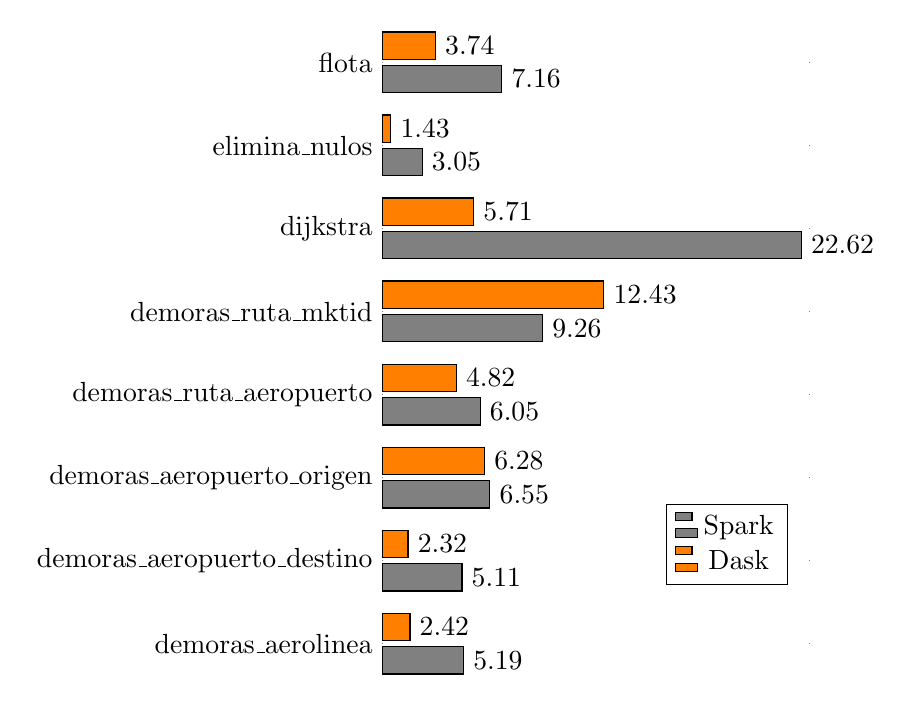
\begin{tikzpicture}
  \begin{axis}[
    xbar,
    y axis line style = { opacity = 0 },
    axis x line       = none,
    y                 = 30,
    x                 = 7,
    legend style={at={(0.95,0.25)}},
    clip              = false,
    tickwidth         = 0.1pt,
    ytick             = data,
    enlarge y limits  = 0.02,
    enlarge x limits  = 0.02,
    symbolic y coords = {demoras\_aerolinea, demoras\_aeropuerto\_destino, demoras\_aeropuerto\_origen, demoras\_ruta\_aeropuerto, demoras\_ruta\_mktid, dijkstra, elimina\_nulos, flota},
    nodes near coords,
  ]
  \addplot[fill=gray] coordinates { (5.187,demoras\_aerolinea)
  						(5.107,demoras\_aeropuerto\_destino)
  						(6.55,demoras\_aeropuerto\_origen)
  						(6.046,demoras\_ruta\_aeropuerto)
  						(9.264,demoras\_ruta\_mktid)
  						(22.62,dijkstra)
  						(3.048,elimina\_nulos)
  						(7.16,flota)};  
  
  \addplot[fill=orange] coordinates { (2.422,demoras\_aerolinea)
  						(2.321,demoras\_aeropuerto\_destino)
  						(6.275,demoras\_aeropuerto\_origen)
  						(4.816,demoras\_ruta\_aeropuerto)
  						(12.429,demoras\_ruta\_mktid)
  						(5.713,dijkstra)
  						(1.433,elimina\_nulos)
  						(3.737,flota)};
                         
  \legend{Spark, Dask}
  \end{axis}
\end{tikzpicture}
\caption{Duración de los procesos con 100,000 registros}
\label{barras:duracion100K}
\end{figure}
\end{center}

\begin{itemize}
	\item \textbf{Robustez} Con esta cantidad de datos, ambos \textit{frameworks} tuvieron resultados satisfactorios en la ejecución de sus procesos sin fallos por lo que uno sigue sin superar al otro en este rubro.
	
	\item \textbf{Variación} En esta ejecución, la desviación estándar fue casi siempre menor a 1 segundo en ambos \textit{frameworks} con algunas excepciones, como se muestra en la tabla \ref{table:duracion100K}. La variación más grande la presentó \textit{Spark} que alcanzó un coeficiente de variación de 1.07 en el proceso \textit{dijkstra}, no obstante, \textit{Dask} tuvo mayor variación en 5 de los 8 procesos, sin embargo, la mayor parte de las veces los procesos tuvieron un coeficiente de variación menor a 0.04 por lo que, en general, la variación fue pequeña en ambos.
	
	\item \textbf{Inicio de la ejecución} La tabla \ref{table:otros100K} muestra que el tiempo de inicio de la ejecución de \textit{Dask} es significativamente menor al de \textit{Spark}, ya que el del primero es menor a 0.01 segundos en casi todos los casos (a excepción del proceso \texttt{dijkstra}) y en el caso de \textit{Spark} es de alrededor de 1 segundo en todos los casos, por lo que el comportamiento se mantiene respecto a la muestra anterior.
	
	\item \textbf{Escritura} De acuerdo a los tiempos de escritura, \textit{Spark} fue más rápido en la escritura a \textit{MySQL} en dos de los cuatro procesos que usan este tipo de escritura (haciéndolo en menos del 63\% del tiempo que le tomó a \textit{Dask}) y con un desempeño similar en dos procesos, en uno de los cuales la diferencia fue menor a 0.1 segundos (\texttt{flota}) y en el otro menor a 0.4 segundos (\texttt{dijkstra}). Esto cambió respecto a las ejecuciones con la muestra anterior donde \textit{Dask} fue más rápido. Por otro lado, \textit{Dask} registró un menor tiempo de escritura a archivos \texttt{parquet} (haciéndolo en menos del 30\% del tiempo que le tomó a \textit{Spark}) en todos los procesos lo cual coincide con el comportamiento de la muestra anterior. Esta información está en la tabla \ref{table:write100K}.
	
	\item \textbf{Capacidad de cómputo} La tabla \ref{table:otros100K} muestra cómo \textit{Dask} logró un menor tiempo de ejecución promedio en prácticamente todos los procesos con la excepción de \texttt{demoras\_ruta\_aeropuerto} y \texttt{demoras\_ruta\_mktid}, los procesos que generan una nueva llave durante la ejecución y en los que los tiempos fueron tan solo entre 3\% y 8\% mayores que los registrados en \textit{Spark}. Además, se mantuvo la diferencia importante en \texttt{dijkstra} (casi 4 veces más tardado en \textit{Spark}) y los demás procesos registraron tiempos promedio entre 80\% y 176\% mayores a \textit{Dask}.
	
	\item \textbf{Duración} La gráfica \ref{barras:duracion100K} permite ver que, a excepción del proceso \texttt{demoras\_ruta\_mktid}, \textit{Dask} fue superior a \textit{Spark} en cuanto a la rapidez de ejecución de los procesos. Las menores diferencias de tiempo entre ambos \textit{frameworks} se registraron en el proceso \texttt{demoras\_aeropuerto\_origen} que consiste de un conteo y obtención del valor mínimo. La diferencia de tiempo parece estar influenciada por la escritura más rápida de \textit{Spark} a \textit{MySQL}, ya que en el proceso \texttt{demoras\_aeropuerto\_destino} la diferencia se incrementa a pesar de ser un proceso muy similar, con las diferencias de que hace la agregación a partir del aeropuerto de origen y no el de destino, calcula el mínimo en lugar del máximo y escribe a \texttt{parquet} en lugar de \textit{MySQL}. También es importante notar que el proceso \texttt{demoras\_ruta\_aeropuerto} tuvo un mayor tiempo total de ejecución a pesar de que su tiempo de cómputo fue menor, lo que muestra, una vez más, la importancia en la rapidez de escritura. Adicionalmente, el tiempo de ejecución del proceso \texttt{dijkstra} fue casi 4 veces mayor que el de \textit{Spark}.


\end{itemize}

\begin{table}
    \centering
    \resizebox{\textwidth}{!}{
    \begin{tabular}{|l|c c c c c c c|}
    \hline
        \multicolumn{1}{|p{2.2cm}|}{\centering \textbf{proceso}} & \multicolumn{1}{p{2.2cm}}{\centering \textbf{framework}} & \multicolumn{1}{p{2.2cm}}{\centering \textbf{número de ejecuciones}} & \multicolumn{1}{p{2.2cm}}{\centering \textbf{duración promedio}} & \multicolumn{1}{p{2.2cm}}{\centering \textbf{desviación estándar}} & \multicolumn{1}{p{2.5cm}}{\centering \textbf{coeficiente de variación}} & \multicolumn{1}{p{2.2cm}}{\centering \textbf{$\frac{\texttt{dask}}{\texttt{spark}}$ (duración)}} & \multicolumn{1}{p{2.2cm}|}{\centering \textbf{$\frac{\texttt{spark}}{\texttt{dask}}$ (duración)}} \\ \hline
        demoras\_aerolinea & dask & 100 & 2.422 & 1.351 & 0.558 & 0.467 & 2.142 \\ % \hline
        demoras\_aerolinea & spark & 100 & 5.187 & 0.384 & 0.074 & 0.467 & 2.142 \\ % \hline
        demoras\_aeropuerto\_destino & dask & 100 & 2.321 & 0.068 & 0.029 & 0.454 & 2.2 \\ % \hline
        demoras\_aeropuerto\_destino & spark & 100 & 5.107 & 0.089 & 0.017 & 0.454 & 2.2 \\ % \hline
        demoras\_aeropuerto\_origen & dask & 100 & 6.275 & 0.128 & 0.02 & 0.958 & 1.044 \\ % \hline
        demoras\_aeropuerto\_origen & spark & 100 & 6.55 & 0.262 & 0.04 & 0.958 & 1.044 \\ % \hline
        demoras\_ruta\_aeropuerto & dask & 100 & 4.816 & 0.131 & 0.027 & 0.797 & 1.255 \\ % \hline
        demoras\_ruta\_aeropuerto & spark & 100 & 6.046 & 0.093 & 0.015 & 0.797 & 1.255 \\ % \hline
        demoras\_ruta\_mktid & dask & 100 & 12.429 & 0.309 & 0.025 & 1.342 & 0.745 \\ % \hline
        demoras\_ruta\_mktid & spark & 100 & 9.264 & 0.337 & 0.036 & 1.342 & 0.745 \\ % \hline
        dijkstra & dask & 100 & 5.713 & 2.683 & 0.47 & 0.253 & 3.959 \\ % \hline
        dijkstra & spark & 100 & 22.62 & 24.204 & 1.07 & 0.253 & 3.959 \\ % \hline
        elimina\_nulos & dask & 100 & 1.433 & 0.085 & 0.06 & 0.47 & 2.127 \\ % \hline
        elimina\_nulos & spark & 100 & 3.048 & 0.054 & 0.018 & 0.47 & 2.127 \\ % \hline
        flota & dask & 100 & 3.737 & 0.146 & 0.039 & 0.522 & 1.916 \\ % \hline
        flota & spark & 100 & 7.16 & 0.147 & 0.021 & 0.522 & 1.916 \\ \hline
    \end{tabular}}
    \caption{Información sobre la duración total con muestra de 100 mil registros.}
    \label{table:duracion100K}
\end{table}


\begin{table}
    \centering
    \resizebox{\textwidth}{!}{
    \begin{tabular}{|l|c c c c c|}
    \hline
        \multicolumn{1}{|p{2.2cm}|}{\centering \textbf{proceso}} & \multicolumn{1}{p{2.2cm}}{\centering \textbf{framework}} & \multicolumn{1}{p{2.2cm}}{\centering \textbf{tiempo de inicio}} & \multicolumn{1}{p{2.2cm}}{\centering \textbf{tiempo de cómputo}} & \multicolumn{1}{p{2.2cm}}{\centering \textbf{$\frac{\texttt{dask}}{\texttt{spark}}$ (cómputo)}} & \multicolumn{1}{p{2.2cm}|}{\centering \textbf{$\frac{\texttt{spark}}{\texttt{dask}}$ (cómputo)}} \\ \hline
        demoras\_aerolinea & dask & 0.009 & 2.217 & 1.82 & 0.549 \\ % \hline
        demoras\_aerolinea & spark & 1.325 & 4.036 & 1.82 & 0.549 \\ % \hline
        demoras\_aeropuerto\_destino & dask & 0.009 & 2.072 & 1.905 & 0.525 \\ % \hline
        demoras\_aeropuerto\_destino & spark & 0.964 & 3.947 & 1.905 & 0.525 \\ % \hline
        demoras\_aeropuerto\_origen & dask & 0.008 & 2.085 & 1.899 & 0.527 \\ % \hline
        demoras\_aeropuerto\_origen & spark & 1.027 & 3.96 & 1.899 & 0.527 \\ % \hline
        demoras\_ruta\_aeropuerto & dask & 0.008 & 4.34 & 0.965 & 1.036 \\ % \hline
        demoras\_ruta\_aeropuerto & spark & 0.957 & 4.188 & 0.965 & 1.036 \\ % \hline
        demoras\_ruta\_mktid & dask & 0.008 & 5.03 & 0.926 & 1.08 \\ % \hline
        demoras\_ruta\_mktid & spark & 0.986 & 4.658 & 0.926 & 1.08 \\ % \hline
        dijkstra & dask & 0.688 & 5.543 & 3.986 & 0.251 \\ % \hline
        dijkstra & spark & 1.022 & 22.093 & 3.986 & 0.251 \\ % \hline
        elimina\_nulos & dask & 0.009 & 1.433 & 2.127 & 0.47 \\ % \hline
        elimina\_nulos & spark & 0.964 & 3.048 & 2.127 & 0.47 \\ % \hline
        flota & dask & 0.009 & 1.907 & 2.758 & 0.363 \\ % \hline
        flota & spark & 1.019 & 5.259 & 2.758 & 0.363 \\ \hline
    \end{tabular}}
    \caption{Información sobre tiempo de cómputo e inicio de la ejecución con muestra de 100 mil registros.}
    \label{table:otros100K}
\end{table}

\begin{table}
    \centering
    \resizebox{\textwidth}{!}{
    \begin{tabular}{|l|c c c c c|}
    \hline
        \multicolumn{1}{|p{2.2cm}|}{\centering \textbf{proceso}} & \multicolumn{1}{p{2.2cm}}{\centering \textbf{framework}} & \multicolumn{1}{p{2.2cm}}{\centering \textbf{destino de escritura}} & \multicolumn{1}{p{2.2cm}}{\centering \textbf{tiempo de escritura promedio}} & \multicolumn{1}{p{2.2cm}}{\centering \textbf{número de renglones escritos}} & \multicolumn{1}{p{2.2cm}|}{\centering \textbf{número de columnas escritos}} \\ \hline
        demoras\_aerolinea & spark & parquet & 1.151 & 49439 & 11 \\ % \hline
        demoras\_aerolinea & dask & parquet & 0.205 & 49439 & 11 \\ % \hline
        demoras\_aeropuerto\_destino & spark & parquet & 1.16 & 116746 & 11 \\ % \hline
        demoras\_aeropuerto\_destino & dask & parquet & 0.249 & 116746 & 11 \\ % \hline
        demoras\_aeropuerto\_origen & spark & mysql & 2.59 & 116656 & 11 \\ % \hline
        demoras\_aeropuerto\_origen & dask & mysql & 4.19 & 116656 & 11 \\ % \hline
        demoras\_ruta\_aeropuerto & spark & parquet & 1.858 & 297814 & 11 \\ % \hline
        demoras\_ruta\_aeropuerto & dask & parquet & 0.476 & 297814 & 11 \\ % \hline
        demoras\_ruta\_mktid & spark & mysql & 4.606 & 267505 & 11 \\ % \hline
        demoras\_ruta\_mktid & dask & mysql & 7.399 & 267505 & 11 \\ % \hline
        dijkstra & spark & mysql & 0.527 & Variable & Variable \\ % \hline
        dijkstra & dask & mysql & 0.17 & Variable & Variable \\ % \hline
        elimina\_nulos & spark & sin escritura & NA & NA & NA \\ % \hline
        elimina\_nulos & dask & sin escritura & NA & NA & NA \\ % \hline
        flota & spark & mysql & 1.901 & 49439 & 6 \\ % \hline
        flota & dask & mysql & 1.83 & 49439 & 6 \\ \hline
    \end{tabular}}
    \caption{Información sobre tiempo de escritura y tamaño del resultado con muestra de 100 mil registros.}
    \label{table:write100K}
\end{table}

En conclusión, para esta muestra de datos, \textit{Dask} mantuvo el mejor desempeño en cuatro rubros: primero, el tiempo de ejecución que no mantuvo en todos los procesos pero sí en 7 de 8, después, en el tiempo de cómputo donde fue superado por \textit{Spark} en 2 casos pero mantuvo el resto, en tercer lugar, el tiempo de escritura a archivos \texttt{parquet} donde fue más rápido en todos los casos y con un margen considerable, y en cuarto lugar el tiempo de inicio de la ejecución que fue muy similar al de la muestra anterior. Por otro lado, \textit{Spark} fue superior en la escritura a \textit{MySQL} en dos de los procesos y en los otros tuvo un desempeño similar a \textit{Dask}. Además, \textit{Spark} tuvo una menor variación en muchos de los procesos pero en ambos \textit{frameworks} fue pequeña. Por último, ambas herramientas parecen ser igual de robustas ya que no tuvieron errores con este número de datos. 


\subsection{Ejecución local con 1,000,000 de registros}

Al pasar a la muestra de un millón de datos la dinámica fue algo distinta y estas son las conclusiones más importantes:

\begin{center}
\begin{figure}
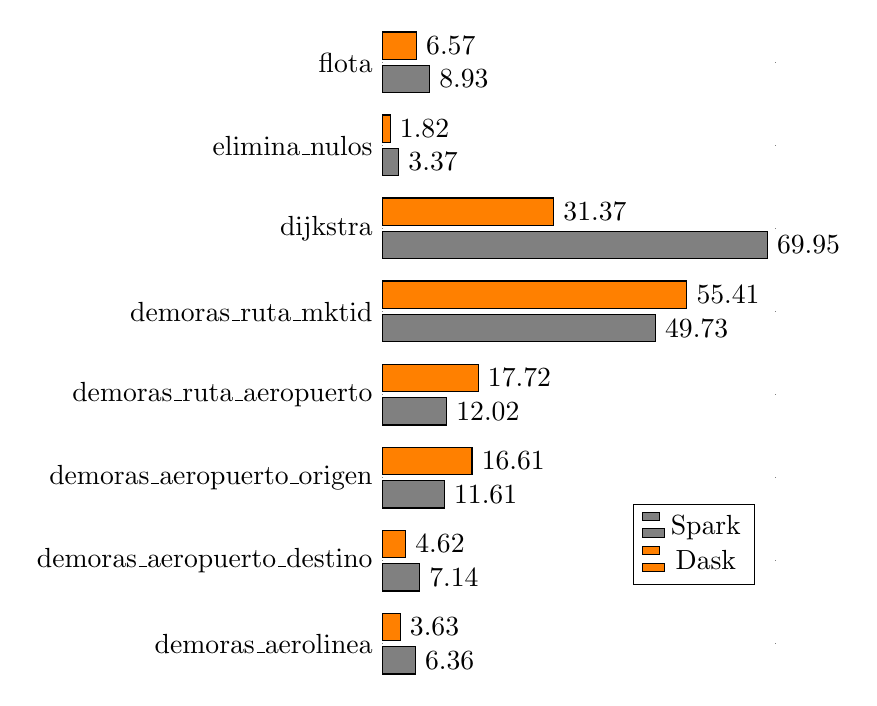
\begin{tikzpicture}
  \begin{axis}[
    xbar,
    y axis line style = { opacity = 0 },
    axis x line       = none,
    y                 = 30,
    x                 = 2,
    legend style={at={(0.95,0.25)}},
    clip              = false,
    tickwidth         = 0.1pt,
    ytick             = data,
    enlarge y limits  = 0.02,
    enlarge x limits  = 0.02,
    symbolic y coords = {demoras\_aerolinea, demoras\_aeropuerto\_destino, demoras\_aeropuerto\_origen, demoras\_ruta\_aeropuerto, demoras\_ruta\_mktid, dijkstra, elimina\_nulos, flota},
    nodes near coords,
  ]
  
  \addplot[fill=gray] coordinates { (6.363,demoras\_aerolinea)
  						(7.137,demoras\_aeropuerto\_destino)
  						(11.607,demoras\_aeropuerto\_origen)
  						(12.019,demoras\_ruta\_aeropuerto)
  						(49.728,demoras\_ruta\_mktid)
  						(69.953,dijkstra)
  						(3.365,elimina\_nulos)
  						(8.932,flota)};  
  
  \addplot[fill=orange] coordinates { (3.629,demoras\_aerolinea)
  						(4.617,demoras\_aeropuerto\_destino)
  						(16.611,demoras\_aeropuerto\_origen)
  						(17.721,demoras\_ruta\_aeropuerto)
  						(55.405,demoras\_ruta\_mktid)
  						(31.371,dijkstra)
  						(1.817,elimina\_nulos)
  						(6.57,flota)};
                         
  \legend{Spark, Dask}
  \end{axis}
\end{tikzpicture}
\caption{Duración de los procesos con 1,000,000 de registros}
\label{barras:duracion1M}
\end{figure}
\end{center}

\begin{itemize}
	\item \textbf{Robustez} Ambos procesos lograron terminar el 100\% de sus ejecuciones por lo que siguen siendo igual de confiables.
	
	\item \textbf{Variación} En estas ejecuciones \textit{Dask} tuvo una variación mayor en 4 de los 8 procesos con diferencias pequeñas respecto a \textit{Spark}. Una vez más, el proceso con mayor variación para \textit{Spark} fue \texttt{dijkstra} con un coeficiente de variación de 1.344 y con todos los demás menores a 0.06. \textit{Dask}, por su parte, tuvo dos procesos con coeficiente mayor a 0.14 siendo \texttt{demoras\_aeropuerto\_destino} el proceso con mayor variación con un coeficiente de 0.289. Esta información se puede ver en la tabla \ref{table:duracion1M}.
	
	\item \textbf{Inicio de la ejecución} Como se aprecia en la tabla \ref{table:otros1M}, en esta muestra \textit{Spark} presentó un incremento en el tiempo de inicio de la ejecución mientras que \textit{Dask} mantuvo un comportamiento similar a muestras previas. 
	
	\item \textbf{Escritura} De acuerdo a los resultados presentados en la tabla \ref{table:write1M}, la superioridad de \textit{Dask} en la velocidad de escritura a \texttt{parquet} se mantuvo, mientras que la superioridad de escritura de \textit{Spark} a \textit{MySQL} se reduce respecto a la muestra anterior ya que sólo es más rápido en dos de los procesos: primero en \texttt{demoras\_aeropuerto\_origen} donde el tiempo de escritura es de casi la mitad del tiempo que el de \textit{Dask}, y en segundo lugar el proceso \texttt{flota} donde la diferencia es mínima, además, la diferencia en el proceso \texttt{demoras\_ruta\_aeropuerto} es mucho menor y favorable a \textit{Dask} cuando en la muestra pasada \textit{Spark} había sido significativamente más rápido. 
	
	\item \textbf{Capacidad de cómputo} Al igual que en la muestra anterior, \textit{Spark} fue más rápido sólo en los procesos \texttt{demoras\_ruta\_aeropuerto} y \texttt{demoras\_ruta\_mktid} en los que \textit{Dask} alcanzó tiempos entre 80\% y 148\% mayores. En \texttt{dijkstra}, \textit{Dask} mantuvo un desempeño mayor aunque \textit{Spark} fue sólo un 123\% más tardado, lo cual es una mejora importante respecto a los resultados de la muestra anterior, sin embargo la necesidad de \textit{Spark} de escribir a disco en cada ejecución sigue dándole una amplia ventaja a \textit{Dask}. Por último, los otros procesos también tuvieron una mejora por parte de \textit{Spark} donde la duración fue entre 29\% y 58\% mayor que es grande, pero mucho menor a las diferencias observadas anteriormente. La evidencia está expuesta en la tabla \ref{table:otros1M}.
	
	\item \textbf{Duración} A pesar de los puntos anteriores, \textit{Spark} redujo la diferencia en el ratio de duración de tiempo en todos los procesos y es más rápido que \textit{Dask} en tres de ellos (\texttt{demoras\_aeropuerto\_origen}, \texttt{demoras\_ruta\_aeropuerto} y \texttt{demoras\_ruta\_mktid}), dos más que en la ejecución anterior. Esto se puede ver en los datos de la tabla \ref{table:duracion1M}. Además, la gráfica \ref{barras:duracion1M}, muestra que la diferencia en el tiempo de ejecución se redujo a menos del 80\% en todos los procesos (a excepción de \texttt{dijkstra}), cuando en la ejecución pasada muchos fueron más de 100\% más tardados.

\end{itemize}

\begin{table}
    \centering
    \resizebox{\textwidth}{!}{
    \begin{tabular}{|l|c c c c c c c|}
    \hline
        \multicolumn{1}{|p{2.2cm}|}{\centering \textbf{proceso}} & \multicolumn{1}{p{2.2cm}}{\centering \textbf{framework}} & \multicolumn{1}{p{2.2cm}}{\centering \textbf{número de ejecuciones}} & \multicolumn{1}{p{2.2cm}}{\centering \textbf{duración promedio}} & \multicolumn{1}{p{2.2cm}}{\centering \textbf{desviación estándar}} & \multicolumn{1}{p{2.5cm}}{\centering \textbf{coeficiente de variación}} & \multicolumn{1}{p{2.2cm}}{\centering \textbf{$\frac{\texttt{dask}}{\texttt{spark}}$ (duración)}} & \multicolumn{1}{p{2.2cm}|}{\centering \textbf{$\frac{\texttt{spark}}{\texttt{dask}}$ (duración)}} \\ \hline
        demoras\_aerolinea & dask & 100 & 3.629 & 0.06 & 0.017 & 0.57 & 1.753 \\ % \hline
        demoras\_aerolinea & spark & 100 & 6.363 & 0.093 & 0.015 & 0.57 & 1.753 \\ % \hline
        demoras\_aeropuerto\_destino & dask & 100 & 4.617 & 1.337 & 0.289 & 0.647 & 1.546 \\ % \hline
        demoras\_aeropuerto\_destino & spark & 100 & 7.137 & 0.418 & 0.058 & 0.647 & 1.546 \\ % \hline
        demoras\_aeropuerto\_origen & dask & 100 & 16.611 & 0.205 & 0.012 & 1.431 & 0.699 \\ % \hline
        demoras\_aeropuerto\_origen & spark & 100 & 11.607 & 0.488 & 0.042 & 1.431 & 0.699 \\ % \hline
        demoras\_ruta\_aeropuerto & dask & 100 & 17.721 & 0.584 & 0.033 & 1.474 & 0.678 \\ % \hline
        demoras\_ruta\_aeropuerto & spark & 100 & 12.019 & 0.196 & 0.016 & 1.474 & 0.678 \\ % \hline
        demoras\_ruta\_mktid & dask & 100 & 55.405 & 0.564 & 0.01 & 1.114 & 0.898 \\ % \hline
        demoras\_ruta\_mktid & spark & 100 & 49.728 & 0.851 & 0.017 & 1.114 & 0.898 \\ % \hline
        dijkstra & dask & 100 & 31.371 & 4.527 & 0.144 & 0.448 & 2.23 \\ % \hline
        dijkstra & spark & 100 & 69.953 & 94.048 & 1.344 & 0.448 & 2.23 \\ % \hline
        elimina\_nulos & dask & 100 & 1.817 & 0.039 & 0.021 & 0.54 & 1.852 \\ % \hline
        elimina\_nulos & spark & 100 & 3.365 & 0.043 & 0.013 & 0.54 & 1.852 \\ % \hline
        flota & dask & 100 & 6.57 & 0.093 & 0.014 & 0.736 & 1.36 \\ % \hline
        flota & spark & 100 & 8.932 & 0.175 & 0.02 & 0.736 & 1.36 \\ \hline
    \end{tabular}}
    \caption{Información sobre la duración total con muestra de 1 millón de registros.}
    \label{table:duracion1M}
\end{table}


\begin{table}
    \centering
    \resizebox{\textwidth}{!}{
    \begin{tabular}{|l|c c c c c|}
    \hline
        \multicolumn{1}{|p{2.2cm}|}{\centering \textbf{proceso}} & \multicolumn{1}{p{2.2cm}}{\centering \textbf{framework}} & \multicolumn{1}{p{2.2cm}}{\centering \textbf{tiempo de inicio}} & \multicolumn{1}{p{2.2cm}}{\centering \textbf{tiempo de cómputo}} & \multicolumn{1}{p{2.2cm}}{\centering \textbf{$\frac{\texttt{dask}}{\texttt{spark}}$ (cómputo)}} & \multicolumn{1}{p{2.2cm}|}{\centering \textbf{$\frac{\texttt{spark}}{\texttt{dask}}$ (cómputo)}} \\ \hline
        demoras\_aerolinea & dask & 0.008 & 3.381 & 1.518 & 0.659 \\ % \hline
        demoras\_aerolinea & spark & 5.545 & 5.132 & 1.518 & 0.659 \\ % \hline
        demoras\_aeropuerto\_destino & dask & 0.009 & 4.12 & 1.294 & 0.773 \\ % \hline
        demoras\_aeropuerto\_destino & spark & 0.977 & 5.331 & 1.294 & 0.773 \\ % \hline
        demoras\_aeropuerto\_origen & dask & 0.009 & 4.038 & 1.31 & 0.763 \\ % \hline
        demoras\_aeropuerto\_origen & spark & 3.144 & 5.291 & 1.31 & 0.763 \\ % \hline
        demoras\_ruta\_aeropuerto & dask & 0.008 & 15.885 & 0.403 & 2.482 \\ % \hline
        demoras\_ruta\_aeropuerto & spark & 3.769 & 6.401 & 0.403 & 2.482 \\ % \hline
        demoras\_ruta\_mktid & dask & 0.009 & 17.364 & 0.531 & 1.882 \\ % \hline
        demoras\_ruta\_mktid & spark & 3.95 & 9.228 & 0.531 & 1.882 \\ % \hline
        dijkstra & dask & 1.975 & 31.12 & 2.23 & 0.448 \\ % \hline
        dijkstra & spark & 7.847 & 69.412 & 2.23 & 0.448 \\ % \hline
        elimina\_nulos & dask & 0.009 & 1.817 & 1.852 & 0.54 \\ % \hline
        elimina\_nulos & spark & 1.093 & 3.365 & 1.852 & 0.54 \\ % \hline
        flota & dask & 0.009 & 4.389 & 1.574 & 0.635 \\ % \hline
        flota & spark & 0.951 & 6.908 & 1.574 & 0.635 \\ \hline
    \end{tabular}}
    \caption{Información sobre tiempo de cómputo e inicio de la ejecución con muestra de 1 millón de registros.}
    \label{table:otros1M}
\end{table}

\begin{table}
    \centering
    \resizebox{\textwidth}{!}{
    \begin{tabular}{|l|c c c c c|}
    \hline
        \multicolumn{1}{|p{2.2cm}|}{\centering \textbf{proceso}} & \multicolumn{1}{p{2.2cm}}{\centering \textbf{framework}} & \multicolumn{1}{p{2.2cm}}{\centering \textbf{destino de escritura}} & \multicolumn{1}{p{2.2cm}}{\centering \textbf{tiempo de escritura promedio}} & \multicolumn{1}{p{2.2cm}}{\centering \textbf{número de renglones escritos}} & \multicolumn{1}{p{2.2cm}|}{\centering \textbf{número de columnas escritos}} \\ \hline
        demoras\_aerolinea & spark & parquet & 1.231 & 76717 & 11 \\ % \hline
        demoras\_aerolinea & dask & parquet & 0.248 & 76717 & 11 \\ % \hline
        demoras\_aeropuerto\_destino & spark & parquet & 1.806 & 436411 & 11 \\ % \hline
        demoras\_aeropuerto\_destino & dask & parquet & 0.497 & 436411 & 11 \\ % \hline
        demoras\_aeropuerto\_origen & spark & mysql & 6.316 & 436681 & 11 \\ % \hline
        demoras\_aeropuerto\_origen & dask & mysql & 12.573 & 436681 & 11 \\ % \hline
        demoras\_ruta\_aeropuerto & spark & parquet & 5.618 & 1619826 & 11 \\ % \hline
        demoras\_ruta\_aeropuerto & dask & parquet & 1.836 & 1619826 & 11 \\ % \hline
        demoras\_ruta\_mktid & spark & mysql & 40.5 & 1430282 & 11 \\ % \hline
        demoras\_ruta\_mktid & dask & mysql & 38.041 & 1430282 & 11 \\ % \hline
        dijkstra & spark & mysql & 0.541 & Variable & Variable \\ % \hline
        dijkstra & dask & mysql & 0.251 & Variable & Variable \\ % \hline
        elimina\_nulos & spark & sin escritura & NA & NA & NA \\ % \hline
        elimina\_nulos & dask & sin escritura & NA & NA & NA \\ % \hline
        flota & spark & mysql & 2.024 & 76717 & 6 \\ % \hline
        flota & dask & mysql & 2.181 & 76717 & 6 \\ \hline
    \end{tabular}}
    \caption{Información sobre tiempo de escritura y tamaño del resultado con muestra de 1 millón de registros.}
    \label{table:write1M}
\end{table}

En conclusión, podemos ver que al incrementar la muestra de datos la superioridad de \textit{Spark} en la escritura a \textit{MySQL} que parecía existir anteriormente no es tan clara, pero se acentúa su mejor desempeño al operar con una nueva llave. Por otro lado, \textit{Dask} aún conserva la ventaja de la escritura a \texttt{parquet} y es más rápido en la ejecución del proceso (sin contar el tiempo de escritura) en todos los procesos que no requieren de la creación de una nueva llave. Sin embargo, la ventaja respecto a \textit{Spark} se redujo significativamente, esto es especialmente evidente al ver el tiempo de cómputo. En cuanto a la robustez y variación, ambos \textit{frameworks} tienen resultados similares con \textit{Spark} siendo un poco más consistente en la duración de sus ejecuciones. Por último, en el algoritmo iterativo \textit{Dask} sigue teniendo mejor desempeño gracias a su capacidad de mantener en memoria resultados intermedios.

\subsection{Ejecución local con 10,000,000 registros}

\begin{center}
\begin{figure}
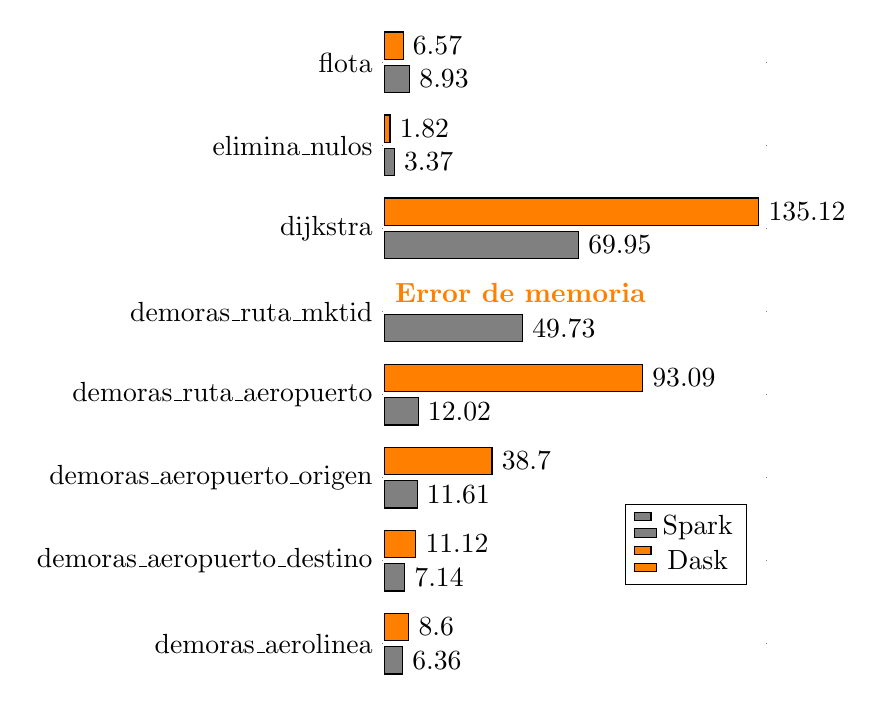
\begin{tikzpicture}
  \begin{axis}[
    xbar,
    y axis line style = { opacity = 0 },
    axis x line       = none,
    y                 = 30,
    x                 = 1,
    legend style={at={(0.95,0.25)}},
    clip              = false,
    tickwidth         = 0.1pt,
    ytick             = data,
    enlarge y limits  = 0.02,
    enlarge x limits  = 0.02,
    symbolic y coords = {demoras\_aerolinea, demoras\_aeropuerto\_destino, demoras\_aeropuerto\_origen, demoras\_ruta\_aeropuerto, demoras\_ruta\_mktid, dijkstra, elimina\_nulos, flota},
    nodes near coords,
  ]
  
  \addplot[fill=gray] coordinates { (6.363,demoras\_aerolinea)
  						(7.137,demoras\_aeropuerto\_destino)
  						(11.607,demoras\_aeropuerto\_origen)
  						(12.019,demoras\_ruta\_aeropuerto)
  						(49.728,demoras\_ruta\_mktid)
  						(69.953,dijkstra)
  						(3.365,elimina\_nulos)
  						(8.932,flota)};
  
  \addplot[fill=orange] coordinates { (8.604,demoras\_aerolinea)
  						(11.123,demoras\_aeropuerto\_destino)
  						(38.7,demoras\_aeropuerto\_origen)
  						(93.087,demoras\_ruta\_aeropuerto)
  						(135.123,dijkstra)
  						(1.817,elimina\_nulos)
  						(6.57,flota)};
                         
  \legend{Spark, Dask}
  % \node[] at (A) {absolute in pgfplots coordinates};
  \end{axis}
  \coordinate (A) at (1.75,4.6);
  \node at (A) {\textbf{\color{orange}{Error de memoria}}};
\end{tikzpicture}
\caption{Duración de los procesos con 10,000,000 de registros.}
\label{barras:duracion10M}
\end{figure}
\end{center}

\begin{itemize}

	\item \textbf{Robustez} En la ejecución de los procesos con esta muestra de datos \textit{Dask} presentó problemas en de falta de memoria en las ejecuciones del proceso \texttt{demoras\_ruta\_mktid} por lo que no completó ninguna de las 100 ejecuciones, algo similar se registró en \cite{comparative-evolution} con un ambiente parecido. El problema de memoria aparece cuando \textit{Dask} calcula el resultado final y lo intenta escribir a \textit{MySQL}. Por el contrario, \textit{Spark} completó el 100\% de las ejecuciones en todos los procesos, por lo que parece escalar de forma más estable y tener una mejor administración del uso de recursos. La evidencia de esto se resume en la tabla \ref{table:duracion10M}.
	
	\item \textbf{Variación} Al ver los resultados de la tabla \ref{table:duracion10M}, observamos que el coeficiente de variación es menor para \textit{Dask} en todos los procesos, por lo que este \textit{framework} es más consistente en sus tiempos de ejecución. Sin embargo, en ambos \textit{frameworks}, el coeficiente es menor a 0.2 en la mayoría de los procesos y las excepciones corresponden a dos procesos de \textit{Spark}: \texttt{dijkstra}, que varía ya que calcula una ruta elegida de forma aleatoria en cada ejecución, y \texttt{elimina\_nulos}, el proceso de menor duración y cuya variación es menor a dos décimas de segundo para \textit{Dask} y menor a 1 segundo para \textit{Spark}, lo que explica el valor alto del coeficiente.
	
	\item \textbf{Inicio de la ejecución} A excepción del proceso \texttt{dijkstra}, el tiempo de inicio de la ejecución sigue siendo mucho menor para \textit{Dask}. Eso se puede ver en la tabla \ref{table:otros10M}.
	
	\item \textbf{Escritura} De acuerdo a los datos expuestos en la tabla \ref{table:write10M}, \textit{Dask} mantiene tiempos menores a los registrados por \textit{Spark} en la escritura de datos a archivos \texttt{parquet}. Por otro lado, \textit{Spark} sigue teniendo un tiempo de escritura menor a \textit{MySQL} en el proceso \texttt{demoras\_aeropuerto\_origen} y un tiempo similar los procesos \texttt{dijkstra} y \texttt{flota}. Del proceso \textit{demoras\_ruta\_mktid} no tenemos información para comparar. 
	
	\item \textbf{Capacidad de cómputo} Al ver el tiempo de cómputo presentado en la tabla \ref{table:otros10M}, vemos que a \textit{Dask} le toma cerca de 17\% más tiempo completar el cálculo de los procesos \texttt{demoras\_aerolinea}, \texttt{demoras\_aeropuerto\_destino} y \texttt{demoras\_aeropuerto\_origen}. Además, en el proceso \texttt{flota}, \textit{Spark} es solo un 1\% más tardado y en el proceso \texttt{demoras\_ruta\_aeropuerto} a \textit{Dask} le tomó casi 6 veces el tiempo que a \textit{Spark} completar el cómputo del resultado. El único proceso en el que \textit{Dask} conserva su superioridad es en \textit{dijkstra} donde su tiempo de ejecución es sólo un 20\% del registrado por \textit{Spark}. 
	
	\item \textbf{Duración} Con loa resultados de esta ejecución, resumida en el gráfico \ref{barras:duracion10M}, observamos que \textit{Spark} sigue siendo más rápido en los procesos \texttt{demoras\_ruta\_aeropuerto} y \texttt{demoras\_aeropuerto\_origen} considerando el tiempo total, en el primer caso con una diferencia mayor que en la muestra anterior y explicada principalmente por el tiempo de cómputo y, en el caso del proceso \texttt{demoras\_aeropuerto\_origen}, la diferencia se debe principalmente a una escritura más rápida por parte de \texttt{Spark} aunque el tiempo de cómputo también es más rápido que en \textit{Dask}. En el caso de los procesos \texttt{demoras\_aerolinea} y \texttt{demoras\_aeropuerto\_destino}, \textit{Dask} registró un menor tiempo promedio de ejecución a pesar de alcanzar valores más altos en el tiempo de cómputo, por lo que la ventaja de escritura a \texttt{parquet} sobre \textit{Spark} sigue siendo un factor importante en su superioridad sobre \textit{Spark} en el tiempo global de ejecución. Aún así, estos dos procesos tuvieron tiempos 4\% y 19\% mayores en \textit{Spark}, respectivamente. Por otro lado, el tiempo de ejecución total del proceso \texttt{flota} fue sólo un 1\% mayor en \textit{Dask} que en \textit{Spark} y sus tiempos de escritura y cómputo fueron muy similares. Adicionalmente, los procesos \texttt{elimina\_nulos} y \texttt{dijkstra} siguen siendo muy superiores en \textit{Dask} ya que alcanzaron tiempos 44\% y 407\% superiores en \textit{Spark}, respectivamente. Además, es importante ver que el proceso \texttt{elimina\_nulos} ha incrementado menos de 1 segundo en ambos \textit{frameworks} a pesar de que la muestra de datos es 1000 veces mayor a la original. En este proceso \textit{Dask} ha mantenido la ventaja consistentemente. En suma, \textit{Spark} fue más rápido en 2 procesos de 7 pero tuvo diferencias menores al 4\% en dos más, por lo que la diferencia entre \textit{Dask} y \textit{Spark} se redujo aún más.

\end{itemize}


\begin{table}
    \centering
    \resizebox{\textwidth}{!}{
    \begin{tabular}{|l|c c c c c c c|}
    \hline
        \multicolumn{1}{|p{2.2cm}|}{\centering \textbf{proceso}} & \multicolumn{1}{p{2.2cm}}{\centering \textbf{framework}} & \multicolumn{1}{p{2.2cm}}{\centering \textbf{número de ejecuciones}} & \multicolumn{1}{p{2.2cm}}{\centering \textbf{duración promedio}} & \multicolumn{1}{p{2.2cm}}{\centering \textbf{desviación estándar}} & \multicolumn{1}{p{2.5cm}}{\centering \textbf{coeficiente de variación}} & \multicolumn{1}{p{2.2cm}}{\centering \textbf{$\frac{\texttt{dask}}{\texttt{spark}}$ (duración)}} & \multicolumn{1}{p{2.2cm}|}{\centering \textbf{$\frac{\texttt{spark}}{\texttt{dask}}$ (duración)}} \\ \hline
        demoras\_aerolinea & dask & 100 & 8.604 & 0.057 & 0.007 & 0.959 & 1.043 \\ %\hline
        demoras\_aerolinea & spark & 100 & 8.97 & 0.169 & 0.019 & 0.959 & 1.043 \\ %\hline
        demoras\_aeropuerto\_destino & dask & 100 & 11.123 & 0.12 & 0.011 & 0.838 & 1.194 \\ %\hline
        demoras\_aeropuerto\_destino & spark & 100 & 13.28 & 0.169 & 0.013 & 0.838 & 1.194 \\ %\hline
        demoras\_aeropuerto\_origen & dask & 100 & 38.7 & 1.933 & 0.05 & 1.213 & 0.825 \\ %\hline
        demoras\_aeropuerto\_origen & spark & 100 & 31.913 & 1.287 & 0.04 & 1.213 & 0.825 \\ %\hline
        demoras\_ruta\_aeropuerto & dask & 100 & 93.087 & 6.446 & 0.069 & 2.147 & 0.466 \\ %\hline
        demoras\_ruta\_aeropuerto & spark & 100 & 43.351 & 2.047 & 0.047 & 2.147 & 0.466 \\ %\hline
        demoras\_ruta\_mktid & spark & 100 & 251.942 & 3.392 & 0.013 & NA & NA \\ %\hline
        dijkstra & dask & 8 & 135.123 & 23.95 & 0.177 & 0.197 & 5.071 \\ %\hline
        dijkstra & spark & 5 & 685.227 & 333.386 & 0.487 & 0.197 & 5.071 \\ %\hline
        elimina\_nulos & dask & 100 & 2.941 & 0.119 & 0.041 & 0.692 & 1.446 \\ %\hline
        elimina\_nulos & spark & 100 & 4.253 & 0.95 & 0.223 & 0.692 & 1.446 \\ %\hline
        flota & dask & 100 & 14.304 & 0.125 & 0.009 & 0.991 & 1.01 \\ %\hline
        flota & spark & 100 & 14.44 & 0.27 & 0.019 & 0.991 & 1.01 \\ \hline
    \end{tabular}}
    \caption{Información sobre la duración total con muestra de 10 millones de registros.}
    \label{table:duracion10M}
\end{table}


\begin{table}
    \centering
    \resizebox{\textwidth}{!}{
    \begin{tabular}{|l|c c c c c|}
    \hline
        \multicolumn{1}{|p{2.2cm}|}{\centering \textbf{proceso}} & \multicolumn{1}{p{2.2cm}}{\centering \textbf{framework}} & \multicolumn{1}{p{2.2cm}}{\centering \textbf{tiempo de inicio}} & \multicolumn{1}{p{2.2cm}}{\centering \textbf{tiempo de cómputo}} & \multicolumn{1}{p{2.2cm}}{\centering \textbf{$\frac{\texttt{dask}}{\texttt{spark}}$ (cómputo)}} & \multicolumn{1}{p{2.2cm}|}{\centering \textbf{$\frac{\texttt{spark}}{\texttt{dask}}$ (cómputo)}} \\ \hline
        demoras\_aerolinea & dask & 0.008 & 8.383 & 0.854 & 1.171 \\ % \hline
        demoras\_aerolinea & spark & 1.039 & 7.16 & 0.854 & 1.171 \\ % \hline
        demoras\_aeropuerto\_destino & dask & 0.008 & 10.116 & 0.851 & 1.175 \\ % \hline
        demoras\_aeropuerto\_destino & spark & 0.968 & 8.612 & 0.851 & 1.175 \\ % \hline
        demoras\_aeropuerto\_origen & dask & 0.009 & 10.306 & 0.847 & 1.181 \\ % \hline
        demoras\_aeropuerto\_origen & spark & 1.033 & 8.729 & 0.847 & 1.181 \\ % \hline
        demoras\_ruta\_aeropuerto & dask & 0.009 & 78.139 & 0.173 & 5.769 \\ % \hline
        demoras\_ruta\_aeropuerto & spark & 0.963 & 13.544 & 0.173 & 5.769 \\ % \hline
        demoras\_ruta\_mktid & spark & 1.208 & 29.576 & NA & NA \\ % \hline
        dijkstra & dask & 8.629 & 134.453 & 5.09 & 0.196 \\ % \hline
        dijkstra & spark & 1.867 & 684.422 & 5.09 & 0.196 \\ % \hline
        elimina\_nulos & dask & 0.009 & NA & NA & NA \\ % \hline
        elimina\_nulos & spark & 1.039 & NA & NA & NA \\ % \hline
        flota & dask & 0.009 & 12.158 & 1.011 & 0.99 \\ % \hline
        flota & spark & 0.972 & 12.286 & 1.011 & 0.99 \\  \hline
    \end{tabular}}
    \caption{Información sobre tiempo de cómputo e inicio de la ejecución con muestra de 10 millones de registros.}
    \label{table:otros10M}
\end{table}

\begin{table}
    \centering
    \resizebox{\textwidth}{!}{
    \begin{tabular}{|l|c c c c c|}
    \hline
        \multicolumn{1}{|p{2.2cm}|}{\centering \textbf{proceso}} & \multicolumn{1}{p{2.2cm}}{\centering \textbf{framework}} & \multicolumn{1}{p{2.2cm}}{\centering \textbf{destino de escritura}} & \multicolumn{1}{p{2.2cm}}{\centering \textbf{tiempo de escritura promedio}} & \multicolumn{1}{p{2.2cm}}{\centering \textbf{número de renglones escritos}} & \multicolumn{1}{p{2.2cm}|}{\centering \textbf{número de columnas escritos}} \\ \hline
        demoras\_aerolinea & spark & parquet & 1.81 & 78113 & 11 \\ % \hline
        demoras\_aerolinea & dask & parquet & 0.221 & 78113 & 11 \\ % \hline
        demoras\_aeropuerto\_destino & spark & parquet & 4.668 & 1042066 & 11 \\ % \hline
        demoras\_aeropuerto\_destino & dask & parquet & 1.007 & 1042066 & 11 \\ % \hline
        demoras\_aeropuerto\_origen & spark & mysql & 23.184 & 1041665 & 11 \\ % \hline
        demoras\_aeropuerto\_origen & dask & mysql & 28.394 & 1041665 & 11 \\ % \hline
        demoras\_ruta\_aeropuerto & spark & parquet & 29.807 & 8361958 & 11 \\ % \hline
        demoras\_ruta\_aeropuerto & dask & parquet & 14.948 & 8361958 & 11 \\ % \hline
        demoras\_ruta\_mktid & spark & mysql & 222.366 & 6824834 & 11 \\ % \hline
        dijkstra & spark & mysql & 0.805 & variable & variable \\ % \hline
        dijkstra & dask & mysql & 0.67 & variable & variable \\ % \hline
        elimina\_nulos & spark & consola & NA & NA & NA \\ % \hline
        elimina\_nulos & dask & consola & NA & NA & NA \\ % \hline
        flota & spark & mysql & 2.154 & 78113 & 6 \\ % \hline
        flota & dask & mysql & 2.146 & 78113 & 6 \\ \hline
    \end{tabular}}
    \caption{Información sobre tiempo de escritura y tamaño del resultado con muestra de 10 millones de registros.}
    \label{table:write10M}
\end{table}

Sintetizando, con esta muestra de datos \textit{Spark} fue superior en la robustez ya que logró completar todos los procesos y \textit{Dask} presentó problemas de memoria en uno de ellos. \textit{Dask}, por su parte, sigue teniendo un mejor desempeño en la escritura a \texttt{parquet}, en el tiempo de inicio de la ejecución, en el la variación del tiempo de ejecución y en el tiempo total de ejecución, aunque la diferencia con \textit{Spark} se sigue reduciendo. Por otro lado, en el tiempo de cómputo, \textit{Spark} fue más rápido en 3 de los 7 procesos y tuvo un desempeño casi igual en un cuarto, por lo que la superioridad de \textit{Dask} ya no es tan evidente, sin embargo, en los procesos \texttt{dijkstra} y \texttt{elimina\_nulos} sí mantuvo una superioridad importante y con una diferencia mucho mayor que las que presentaron los procesos en los que \textit{Spark} fue más rápido.

\subsection{Ejecución local con 80,000,000 registros}


\subsection{Cambio del desempeño entre muestras}

Después de haber revisado de forma independiente cada muestra, podemos pasar al análisis del comportamiento de cada \textit{framework} a través de las distintas muestras y procesos. Esta sección se centrará en los promedio de tiempo de ejecución registrado y el tiempo de escritura y su dinámica al incrementar el tamaño de los datos a procesar. Primero se hará un análisis de cada proceso individual y después se obtendrán conclusiones generales sobre cada herramienta. En esta sección también se incluye información más detallada sobre el número de registros que escribe cada proceso a sus respectivos destinos (\texttt{parquet} o \textit{MySQL}), y es importante mencionar que es normal que el tamaño del resultado no crezca de forma proporcional al tamaño de los datos que se procesan ya que la mayoría de los procesos tienen datos agregados como resultado final.

\subsubsection{Proceso de cálculo de flota}

Este proceso es uno de los que registró menos tiempo de ejecución en las distintas muestras y uno en el que \textit{Dask} fue superior en la mayoría de las muestras. Sus operaciones más importantes son la eliminación de registros duplicados en una columna y su posterior conteo agrupando por distintas columnas con valores de tiempo. El resultado se escribe a \textit{MySQL}.

La figura \ref{lineas:local-flota} muestra cómo varía la diferencia entre \textit{Dask} y \textit{Spark} al incrementar el número de datos a procesar, empezando por 10,000 y llegando hasta un poco más de 80 millones. En la gráfica es claro como el incremento de tiempo de ambos \textit{frameworks} es pequeño (de entre 8 y 11 segundos) comparado con el número de registros que tiene que procesar. Aunque el cuarto punto corresponde a un conjunto de datos 1000 veces mayor que el tiempo promedio registrado es cercano a 3 veces mayor en el caso de \textit{Spark} y 4 en el caso de \textit{Dask}, lo cuál muestra una importante capacidad de procesamiento de datos con un pequeño incremento de tiempo transcurrido. Sin embargo, esta tendencia se rompe al considerar el total de los datos, ya que el tiempo de ejecución parece crecer de forma proporcional a los datos (tanto los datos como el tiempo de ejecución son 8 veces mayores que en la muestra anterior). 
\begin{figure}
\centering
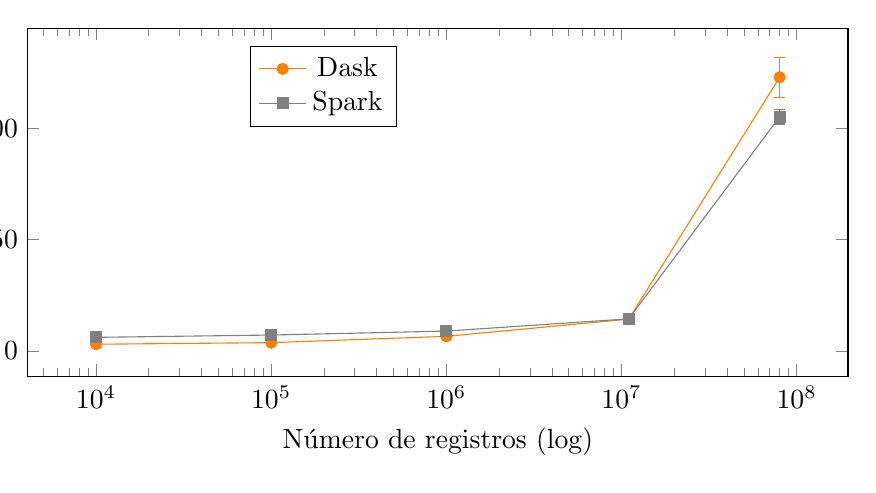
\begin{tikzpicture}[trim axis left, trim axis right]
\begin{axis}[
	xlabel = Número de registros (log),
	ylabel = Duración en segundos,
	legend style={at={(0.45,0.95)}},
	xmode=log,
	% ymode=log,
	width=12cm,
	height=6cm
	]
  \addplot+[orange,mark options={fill=orange},error bars/.cd,y dir=both,y explicit] 
    table[x=x,y=y,y error=error] {
      x   y   error
      10000 3.029 1.308
      100000 3.737 0.146
      1000000 6.57 0.093
      11000000 14.304 0.125
      80000000 122.987 8.984
    };
    
  \addplot+[gray,mark options={fill=gray},error bars/.cd,y dir=both,y explicit] 
    table[x=x,y=y,y error=error] {
      x   y   error
      10000 6.12 0.553
      100000 7.16 0.147
      1000000 8.932 0.175
      11000000 14.44 0.27
      80000000 105.209 3.253
    };
    \legend {Dask, Spark}
\end{axis}
\end{tikzpicture}
\caption{Duración promedio del proceso flota en diferentes muestras.}
\label{lineas:local-flota}
\end{figure}

Al analizar los tiempos de escritura a \textit{MySQL}, representados en \ref{lineas:local-flota-write}, podemos ver que no fue un factor importante para el tiempo de ejecución, ya que el aumento de tiempo de la primera a la última muestra no fue significativo. Además no se observa una mejora clara en el desempeño de ninguna de las herramientas conforme los datos aumentan, en particular, en la muestra de 11 millones, ambos \textit{frameworks} presentan un cambio importante en la tendencia que estaban presentando, \textit{Spark} aumentando significativamente el tiempo de ejecución con un pequeño incremento en el número de registros y \textit{Dask} incluso mejorando el tiempo de escritura a pesar del aumento de registros.

\begin{figure}
\centering
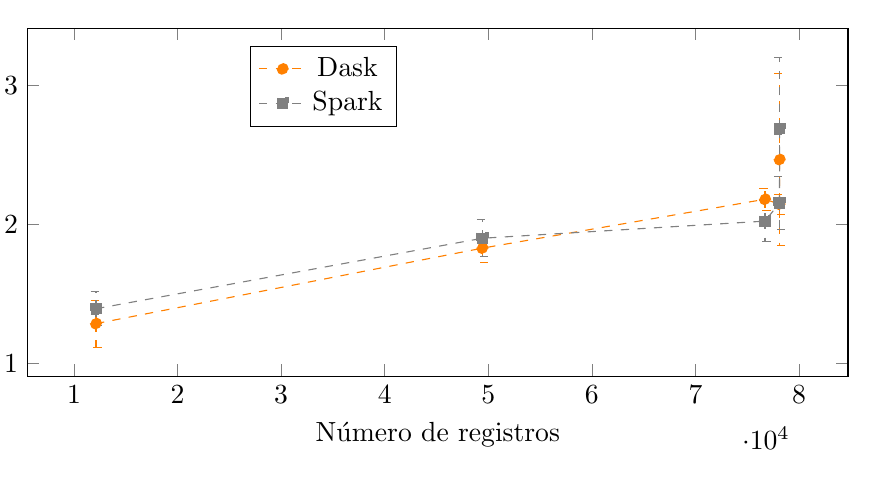
\begin{tikzpicture}[trim axis left, trim axis right]
\begin{axis}[
	xlabel = Número de registros,
	ylabel = Duración en segundos,
	legend style={at={(0.45,0.95)}},
	% xmode=log,
	% ymode=log,
	width=12cm,
	height=6cm
	]
  \addplot+[dashed, orange,mark options={fill=orange},error bars/.cd,y dir=both,y explicit] 
    table[x=x,y=y,y error=error] {
      x   y   error
      12135 1.288 0.169
      49439 1.83 0.101
      76717 2.181 0.079
      78113 2.146 0.072
      78133 2.466 0.619
       
    };
    
  \addplot+[dashed, gray,mark options={fill=gray},error bars/.cd,y dir=both,y explicit] 
    table[x=x,y=y,y error=error] {
      x   y   error
      12135 1.395 0.121
      49439 1.901 0.132
      76717 2.024 0.149
      78113 2.154 0.188
      78133 2.688 0.513
    };
    \legend {Dask, Spark}
\end{axis}
\end{tikzpicture}
\caption{Duración promedio de la escritura de resultados del proceso flota en diferentes muestras.}
\label{lineas:local-flota-write}
\end{figure}

\subsubsection{Proceso de cálculo de demoras por aerolínea}

Este proceso tiene como operaciones principales conteo de una columna y obtención de promedios de otras 5, agrupando respecto a distintas columnas de tiempo. El resultado final se almacena en un archivo \texttt{parquet}.

Al analizar los resultados representados por la figura \ref{lineas:local-demoras-aerolinea}, podemos ver que el incremento de tiempo de la primera a la cuarta muestra es pequeño comparado con el aumento del conjunto de datos (cercano a 1000x), sin embargo, cuando se llega a al última muestra se aprecia un incremento mucho mayor a los observados anteriormente. Adicionalmente, es en la última muestra cuando \textit{Spark} supera el desempeño de \textit{Dask} que se acortaba conforme crecía el número de datos. Con esta información se puede ver cómo \textit{Spark} se vuelve más competitivo conforme aumenta el tamaño del conjunto de datos. 

\begin{figure}
\centering
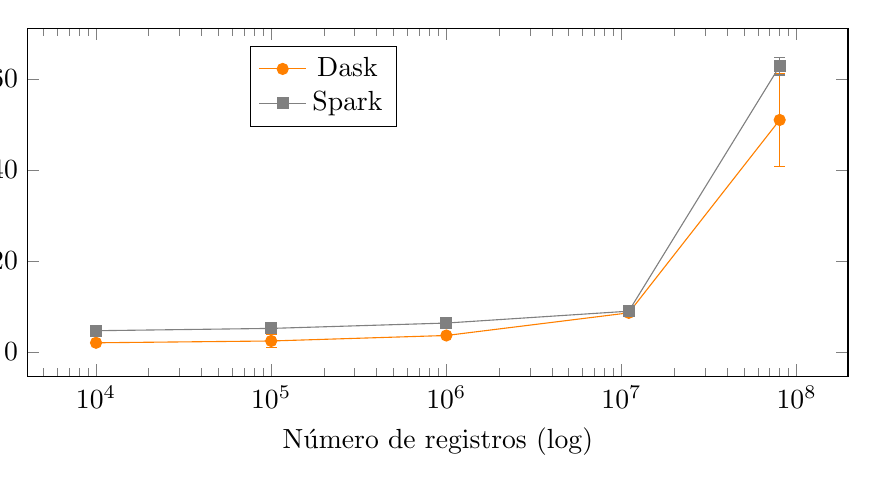
\begin{tikzpicture}[trim axis left, trim axis right]
\begin{axis}[
	xlabel = Número de registros (log),
	ylabel = Duración en segundos,
	legend style={at={(0.45,0.95)}},
	xmode=log,
	% ymode=log,
	width=12cm,
	height=6cm
	]
  \addplot+[orange,mark options={fill=orange},error bars/.cd,y dir=both,y explicit] 
    table[x=x,y=y,y error=error] {
      x   y   error
      10000 2.024 0.048
      100000 2.422 1.351
      1000000 3.629 0.06
      11000000 8.604 0.057
      80000000 50.991 10.137
    };
    
  \addplot+[gray,mark options={fill=gray},error bars/.cd,y dir=both,y explicit] 
    table[x=x,y=y,y error=error] {
      x   y   error
      10000 4.678 0.065
      100000 5.187 0.384
      1000000 6.363 0.093
      11000000 8.97 0.169
      80000000 62.825 1.957
    };
    \legend {Dask, Spark}
\end{axis}
\end{tikzpicture}
\caption{Duración promedio del proceso demoras\_aerolinea en diferentes muestras.}
\label{lineas:local-demoras-aerolinea}
\end{figure}

Por otra parte, analizando los resultados de la escritura, representados por la figura \ref{lineas:local-demoras-aerolinea-write}, podemos ver que el tiempo de escritura de ambos \textit{frameworks} es muy bajo y que \textit{Dask} es especialmente constante en el tiempo de escritura. Sin embargo, considerando el poco tiempo que este proceso toma, la escritura a archivos \textit{parquet} no  es un factor importante en la duración total debido a la velocidad de escritura de ambas herramientas y el bajo incremento del tamaño del \textit{DataFrame} resultante.

\begin{figure}
\centering
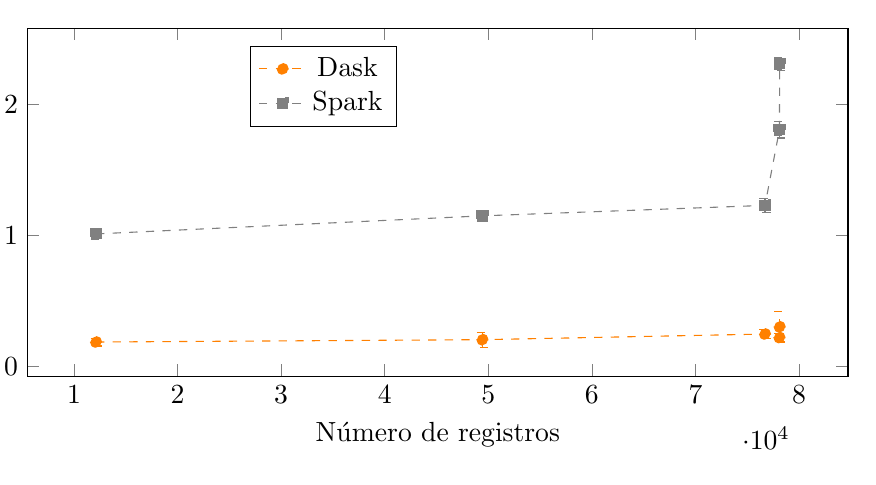
\begin{tikzpicture}[trim axis left, trim axis right]
\begin{axis}[
	xlabel = Número de registros,
	ylabel = Duración en segundos,
	legend style={at={(0.45,0.95)}},
	% xmode=log,
	% ymode=log,
	width=12cm,
	height=6cm
	]
  \addplot+[dashed, orange,mark options={fill=orange},error bars/.cd,y dir=both,y explicit] 
    table[x=x,y=y,y error=error] {
      x   y   error
      12135 0.187 0.03
      49439 0.205 0.057
      76717 0.248 0.037
      78113 0.221 0.031
      78133 0.303 0.118
    };
    
  \addplot+[dashed, gray,mark options={fill=gray},error bars/.cd,y dir=both,y explicit] 
    table[x=x,y=y,y error=error] {
      x   y   error
      12135 1.013 0.03
      49439 1.151 0.042
      76717 1.231 0.056
      78113 1.81 0.064
      78133 2.313 0.05
    };
    \legend {Dask, Spark}
\end{axis}
\end{tikzpicture}
\caption{Duración promedio de escritura de resultados del proceso demoras\_aerolinea en diferentes muestras.}
\label{lineas:local-demoras-aerolinea-write}
\end{figure}

\subsubsection{Proceso de cálculo de demoras por aeropuerto de destino}

Este proceso tiene como operaciones principales el conteo en una columna y la obtención del mínimo de otras 5, agrupando de acuerdo a distintos periodos de tiempo representados en diversas columnas. El resultado del proceso se escribe en un archivo \texttt{parquet}.

Entre la primera y la penúltima muestra, el incremento de tiempo del proceso es de aproximadamente 10 segundos, que se traduce en un tiempo aproximadamente 5 y 2 veces mayor para \textit{Dask} y \textit{Spark} respectivamente, a pesar de que el cuarto conjunto de datos es más de 1000 veces mayor que el de la primera muestra. Esto muestra una gran capacidad para procesar más y más datos con los mismos recursos y poco incremento en el tiempo de ejecución por parte de ambos \textit{frameworks}. Sin embargo esta tendencia se rompe cuando se superan los 80 millones de registros. Especialmente en el caso de \textit{Spark}, el tiempo de ejecución del proceso con la muestra más grande es 60 veces mayor a la muestra más pequeña, mientras que en el caso de \textit{Dask} es 40 veces mayor a la de la menor muestra. Sin embargo, \textit{Dask} tiene un mejor desempeño ya que ejecuta todos los procesos más rápido que \textit{Spark}, con una diferencia de pocos segundos en las primeras cuatro muestras pero con una diferencia importante en la última en la que \textit{Spark} es más de tres veces más tardado. En este caso, \textit{Dask} muestra una mayor capacidad para procesar cantidades de datos cada vez más grandes.

\begin{figure}
\centering
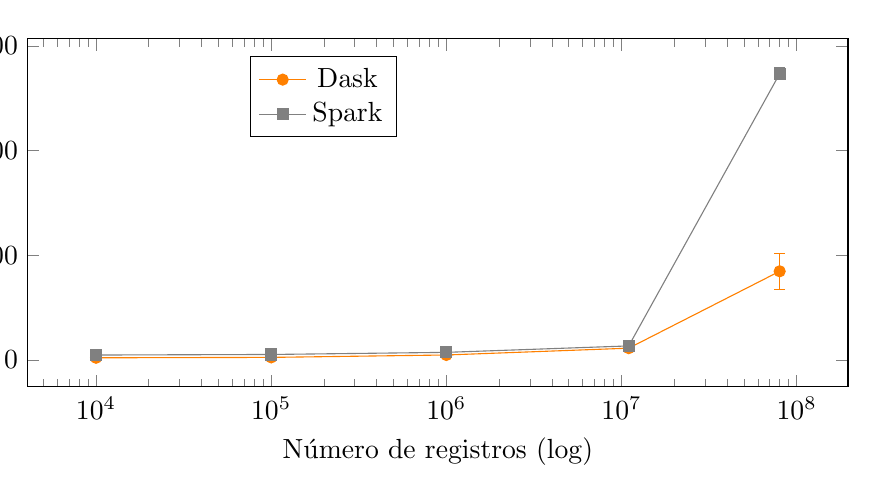
\begin{tikzpicture}[trim axis left, trim axis right]
\begin{axis}[
	xlabel = Número de registros (log),
	ylabel = Duración en segundos,
	legend style={at={(0.45,0.95)}},
	xmode=log,
	% ymode=log,
	width=12cm,
	height=6cm
	]
  \addplot+[orange,mark options={fill=orange},error bars/.cd,y dir=both,y explicit] 
    table[x=x,y=y,y error=error] {
      x   y   error
      10000 1.939 0.043
      100000 2.321 0.068
      1000000 4.617 1.337
      11000000 11.123 0.12
      80000000 84.579 17.202
    };
    
  \addplot+[gray,mark options={fill=gray},error bars/.cd,y dir=both,y explicit] 
    table[x=x,y=y,y error=error] {
      x   y   error
      10000 4.578 0.064
      100000 5.107 0.089
      1000000 7.137 0.418
      11000000 13.28 0.169
      80000000 273.324 5.563
    };
    \legend {Dask, Spark}
\end{axis}
\end{tikzpicture}
\caption{Duración promedio del proceso demoras\_aeropuerto\_destino en diferentes muestras.}
\label{lineas:local-demoras-aeropuerto-destino}
\end{figure}

Al analizar el tiempo de escritura, representado en la gráfica \ref{lineas:local-demoras-aeropuerto-destino-write}, podemos apreciar que conforme crece la muestra de datos \textit{Dask} tiene un menor incremento de tiempo de \textit{Spark}, por lo que la diferencia entre el tiempo de escritura crece con el tiempo. Además, la tendencia observada en la figura \ref{lineas:local-demoras-aeropuerto-destino} es similar a la representada en la gráfica de escritura. Sin embargo, el bajo tiempo de escritura tiene un impacto menor en el tiempo total de ejecución conforme crece el número de datos totales a procesar, por lo que podemos concluir que \textit{Dask} es más rápido para escribir el resultado y también para calcularlo.

\begin{figure}
\centering
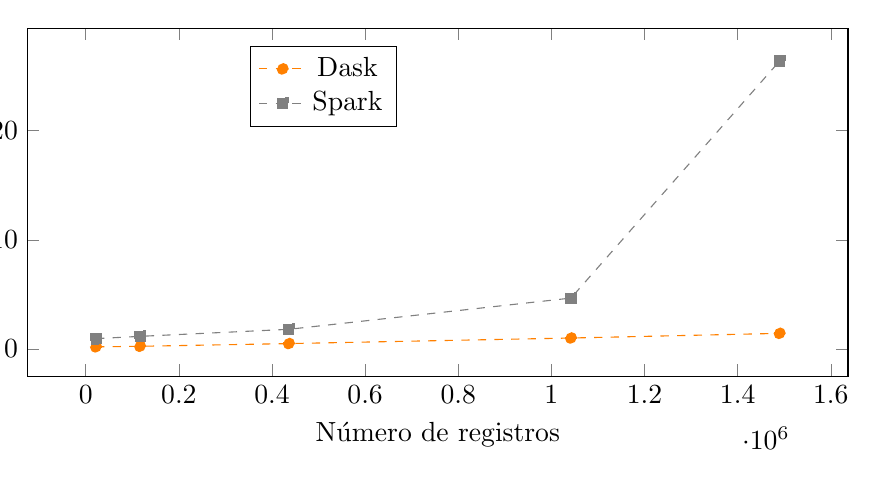
\begin{tikzpicture}[trim axis left, trim axis right]
\begin{axis}[
	xlabel = Número de registros,
	ylabel = Duración en segundos,
	legend style={at={(0.45,0.95)}},
	% xmode=log,
	% ymode=log,
	width=12cm,
	height=6cm
	]
  \addplot+[dashed, orange,mark options={fill=orange},error bars/.cd,y dir=both,y explicit] 
    table[x=x,y=y,y error=error] {
      x   y   error
      22144 0.195 0.024  
      116746 0.249 0.041 
      436411 0.497 0.052 
      1042066 1.007 0.041
      1490152 1.434 0.09
    };
    
  \addplot+[dashed, gray,mark options={fill=gray},error bars/.cd,y dir=both,y explicit] 
    table[x=x,y=y,y error=error] {
      x   y   error
      22144 0.951 0.031  
	  116746 1.16 0.062  
	  436411 1.806 0.057 
	  1042066 4.668 0.083
	  1490152 26.394 0.345
    };
    \legend {Dask, Spark}
\end{axis}
\end{tikzpicture}
\caption{Duración promedio de la escritura de resultados del proceso demoras\_aeropuerto\_destino en diferentes muestras.}
\label{lineas:local-demoras-aeropuerto-destino-write}
\end{figure}

\subsubsection{Proceso de cálculo de demoras por aeropuerto de origen}

Este proceso tiene como operaciones principales el conteo en una columna y la obtención del máximo de otras 5, agrupando de acuerdo a distintos periodos de tiempo representados en diversas columnas. El resultado del proceso se escribe a una base de datos \textit{MySQL}.

Cómo se ve en la figura \ref{lineas:local-demoras-aeropuerto-origen}, en este proceso los \textit{frameworks} tienen un comportamiento similar a través de las distintas muestras. Algo interesante es que, a diferencia de otros procesos, \textit{Spark} supera a \textit{Dask} en desempeño durante las muestras de 1 millón y 11 millones de registros pero \textit{Dask} es más rápido en la última muestra. Además, en la figura \ref{lineas:local-demoras-aeropuerto-origen-write} podemos ver que el tiempo de escritura también se incrementa de forma similar en ambas herramientas y de hecho, \textit{Spark} tiene una mayor capacidad de escritura a \textit{MySQL} que \textit{Dask} aunque la diferencia de tiempo parece mantenerse para las muestras más grandes. Debido a esto último, podemos concluir que la diferencia en el tiempo total de ejecución presentada en la última muestra se debe a un mejor procesamiento de datos por parte de \textit{Dask}, mientras que en las dos muestras anteriores, la superioridad de \textit{Spark} se explica, en parte, por su mayor desempeño en la escritura. 

\begin{figure}
\centering
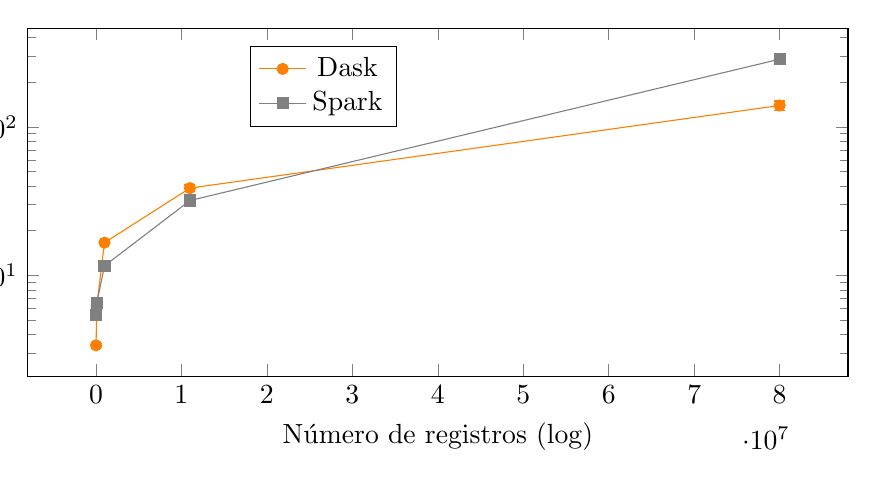
\begin{tikzpicture}[trim axis left, trim axis right]
\begin{axis}[
	xlabel = Número de registros (log),
	ylabel = Duración en segundos,
	legend style={at={(0.45,0.95)}},
	% xmode=log,
	ymode=log,
	width=12cm,
	height=6cm
	]
  \addplot+[orange,mark options={fill=orange},error bars/.cd,y dir=both,y explicit] 
    table[x=x,y=y,y error=error] {
      x   y   error
      10000 3.386 0.095
      100000 6.275 0.128
      1000000 16.611 0.205
      11000000 38.7 1.933
      80000000 139.247 9.893
    };
    
  \addplot+[gray,mark options={fill=gray},error bars/.cd,y dir=both,y explicit] 
    table[x=x,y=y,y error=error] {
      x   y   error
      10000 5.406 0.132
      100000 6.55 0.262
      1000000 11.607 0.488
      11000000 31.913 1.287
      80000000 285.318 8.8
    };
    \legend {Dask, Spark}
\end{axis}
\end{tikzpicture}
\caption{Duración promedio del proceso demoras\_aeropuerto\_origen en diferentes muestras.}
\label{lineas:local-demoras-aeropuerto-origen}
\end{figure}

\begin{figure}
\centering
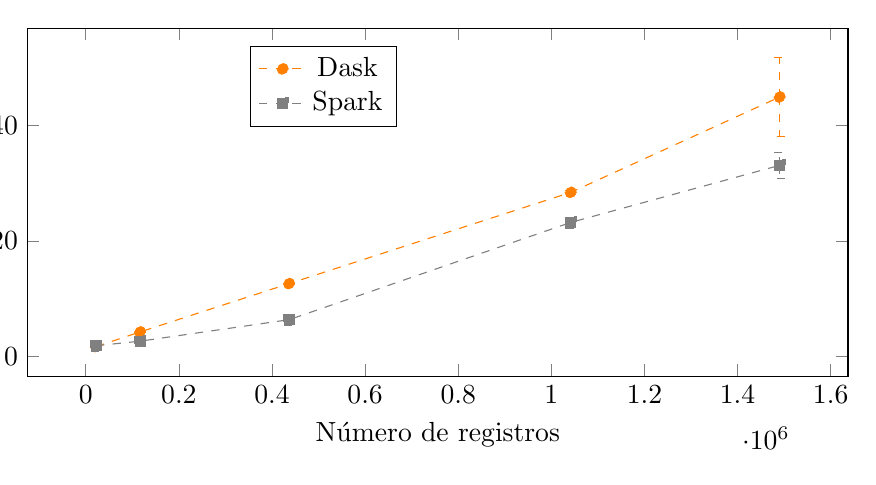
\begin{tikzpicture}[trim axis left, trim axis right]
\begin{axis}[
	xlabel = Número de registros,
	ylabel = Duración en segundos,
	legend style={at={(0.45,0.95)}},
	% xmode=log,
	% ymode=log,
	width=12cm,
	height=6cm
	]
  \addplot+[dashed, orange,mark options={fill=orange},error bars/.cd,y dir=both,y explicit] 
    table[x=x,y=y,y error=error] {
      x   y   error
      22086 1.643 0.087
      116656 4.19 0.119
      436681 12.573 0.189
      1041665 28.394 0.355
      1490410 44.934 6.905
    };
    
  \addplot+[dashed, gray,mark options={fill=gray},error bars/.cd,y dir=both,y explicit] 
    table[x=x,y=y,y error=error] {
      x   y   error
      22086 1.801 0.125 
	  116656 2.59 0.255  
	  436681 6.316 0.479
	  1041665 23.184 0.774
	  1490410 33.087 2.261
    };
    \legend {Dask, Spark}
\end{axis}
\end{tikzpicture}
\caption{Duración promedio de la escritura de resultados del proceso demoras\_aeropuerto\_origen en diferentes muestras.}
\label{lineas:local-demoras-aeropuerto-origen-write}
\end{figure}

\subsubsection{Proceso de cálculo de demoras por ruta entre aeropuertos}

El proceso \texttt{demoras\_ruta\_aeropuertos} tiene como operaciones principales  la creación de una nueva llave a partir de la concatenación de dos columnas existentes y después un conteo en una columna, cálculo del promedio en otras 5, agrupando de acuerdo a la nueva llave y a otras columnas que describen periodos de tiempo. El resultado final se escribe a un archivo \texttt{parquet}.

La figura \ref{lineas:local-demoras-ruta-aeropuerto} muestra como las herramientas tienen un desempeño muy similar en las primeras dos muestras y \textit{Spark} es ligeramente superior a partir de la muestra de 1 millón de datos e incrementa la diferencia significativamente en la muestra de 10 millones de datos. Para la última muestra, \textit{Dask} tiene problemas de memoria que le impiden terminar la ejecución del proceso por lo que \textit{Spark} también tiene un desempeño superior. 

Por otro lado, al observar la figura \ref{lineas:local-demoras-ruta-aeropuerto-write} podemos ver que a \textit{Spark} le toma más tiempo escribir resultados a archivos \texttt{parquet} y a pesar de ello tiene un desempeño superior, por lo que la rapidez de \textit{Spark} viene de su capacidad de procesamiento y creación de una nueva llave.

\begin{figure}
\centering
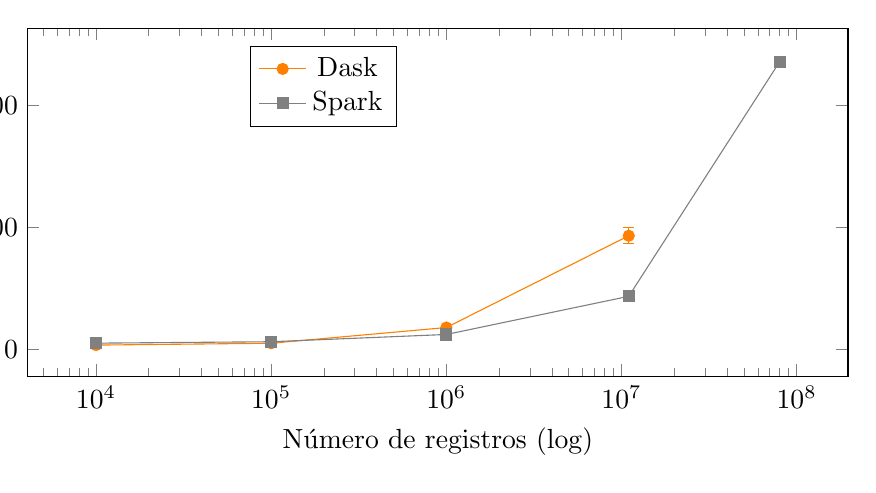
\begin{tikzpicture}[trim axis left, trim axis right]
\begin{axis}[
	xlabel = Número de registros (log),
	ylabel = Duración en segundos,
	legend style={at={(0.45,0.95)}},
	xmode=log,
	% ymode=log,
	width=12cm,
	height=6cm
	]
  \addplot+[orange,mark options={fill=orange},error bars/.cd,y dir=both,y explicit] 
    table[x=x,y=y,y error=error] {
      x   y   error
      10000 3.291 1.688
      100000 4.816 0.131
      1000000 17.721 0.584
      11000000 93.087 6.446
      % 80000000 NA NA
    };
    
  \addplot+[gray,mark options={fill=gray},error bars/.cd,y dir=both,y explicit] 
    table[x=x,y=y,y error=error] {
      x   y   error
      10000 4.881 0.091
      100000 6.046 0.093
      1000000 12.019 0.196
      11000000 43.351 2.047
      80000000 235.991 3.713
    };
    \legend {Dask, Spark}
\end{axis}
\end{tikzpicture}
\caption{Duración promedio del proceso demoras\_ruta\_aeropuerto en diferentes muestras.}
\label{lineas:local-demoras-ruta-aeropuerto}
\end{figure}

\begin{figure}
\centering
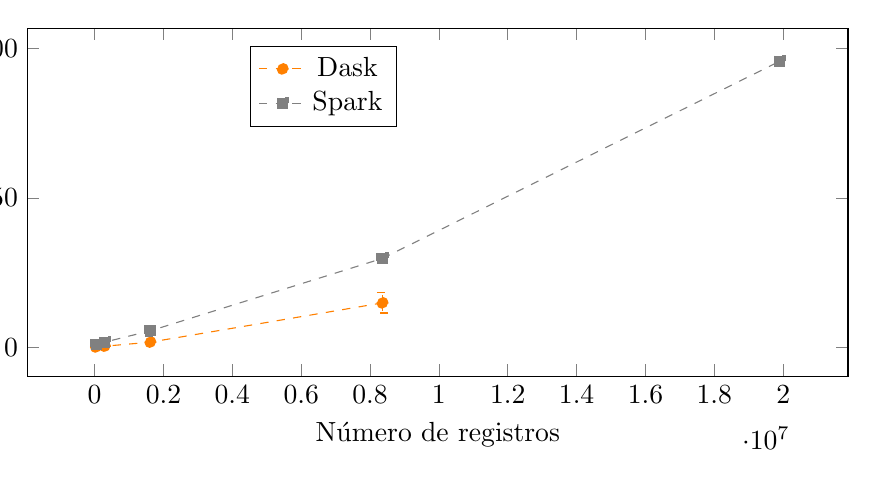
\begin{tikzpicture}[trim axis left, trim axis right]
\begin{axis}[
	xlabel = Número de registros,
	ylabel = Duración en segundos,
	legend style={at={(0.45,0.95)}},
	% xmode=log,
	% ymode=log,
	width=12cm,
	height=6cm
	]
  \addplot+[dashed, orange,mark options={fill=orange},error bars/.cd,y dir=both,y explicit] 
    table[x=x,y=y,y error=error] {
      x   y   error
      41147 0.209 0.046
      297814 0.476 0.047
      1619826 1.836 0.029
      8361958 14.948 3.378
    };
    
  \addplot+[dashed, gray,mark options={fill=gray},error bars/.cd,y dir=both,y explicit] 
    table[x=x,y=y,y error=error] {
      x   y   error
      41147 1.114 0.047
	  297814 1.858 0.088
	  1619826 5.618 0.19
	  8361958 29.807 0.501
	  19897358 95.66 1.355
    };
    \legend {Dask, Spark}
\end{axis}
\end{tikzpicture}
\caption{Duración promedio de la escritura de resultados del proceso demoras\_aeropuerto\_origen en diferentes muestras.}
\label{lineas:local-demoras-ruta-aeropuerto-write}
\end{figure}

\subsubsection{Proceso de cálculo de demoras por ruta entre ciudades}

Este proceso tiene como operaciones principales la creación de una nueva llave a partir de la concatenación de dos columnas existentes y después un conteo en una columna, cálculo de la desviación estándar en otras 5, agrupando de acuerdo a la nueva llave y a otras columnas que describen periodos de tiempo. El resultado final se escribe a un archivo \texttt{parquet}. Es importante mencionar que este es el proceso más demandante de los implementados debido a el tipo de operación que calcula, el número de registros que utiliza, el tamaño de su resultado y la escritura a \textit{MySQL} que ha demostrado ser más costosa que a archivos \texttt{parquet}.

La figura \ref{lineas:local-demoras-ruta-mktid} muestra que al principio, la diferencia entre la rapidez de ejecución de ambos \textit{frameworks} es muy poca, sin embargo, a partir de la muestra de 10 millones de datos, \textit{Dask} tiene problemas de memoria y no logra finalizar la ejecución.

La gráfica \ref{lineas:local-demoras-ruta-mktid} muestra que el tiempo de escritura crece de una forma menos acelerada que el tiempo de ejecución total. Además, es interesante ver cómo en el caso de \textit{Spark} aproximadamente un 40\% del tiempo del tiempo total corresponde al tiempo de escritura. Por otro lado, debido a la falta de información sobre \textit{Dask}, no podemos obtener conclusiones concretas. 

\begin{figure}
\centering
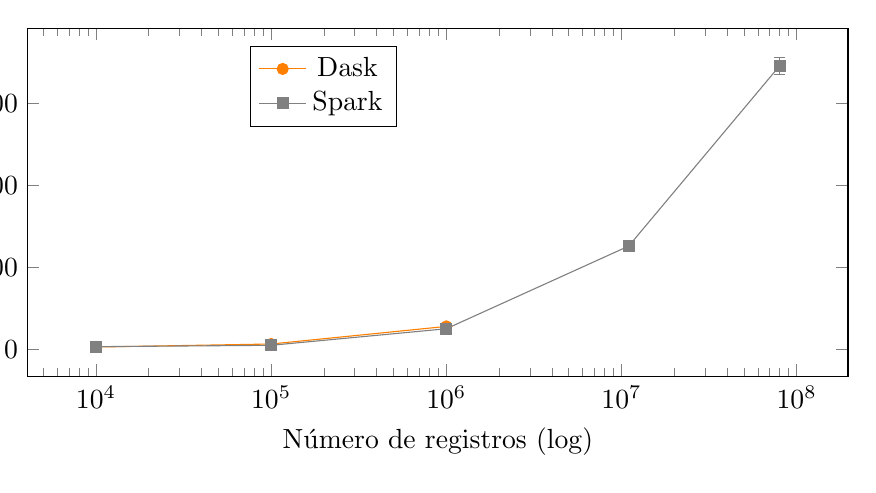
\begin{tikzpicture}[trim axis left, trim axis right]
\begin{axis}[
	xlabel = Número de registros (log),
	ylabel = Duración en segundos,
	legend style={at={(0.45,0.95)}},
	xmode=log,
	% ymode=log,
	width=12cm,
	height=6cm
	]
  \addplot+[orange,mark options={fill=orange},error bars/.cd,y dir=both,y explicit] 
    table[x=x,y=y,y error=error] {
      x   y   error
      10000 4.991 0.252
      100000 12.429 0.309
      1000000 55.405 0.564
      % 11000000 NA NA
      % 80000000 NA NA
    };
    
  \addplot+[gray,mark options={fill=gray},error bars/.cd,y dir=both,y explicit] 
    table[x=x,y=y,y error=error] {
      x   y   error
      10000 5.901 0.135
      100000 9.264 0.337
      1000000 49.728 0.851
      11000000 251.942 3.392
      80000000 692.743 20.908
    };
    \legend {Dask, Spark}
\end{axis}
\end{tikzpicture}
\caption{Duración promedio del proceso demoras\_ruta\_mktid en diferentes muestras.}
\label{lineas:local-demoras-ruta-mktid}
\end{figure}


\begin{figure}
\centering
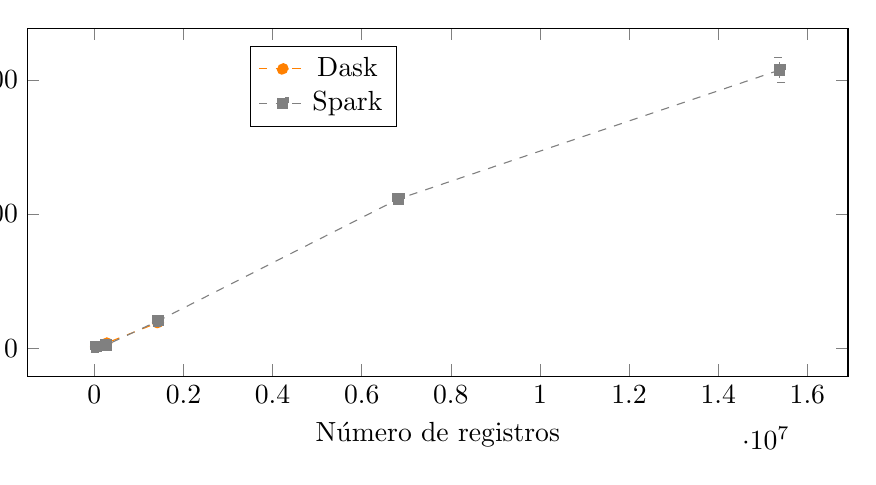
\begin{tikzpicture}[trim axis left, trim axis right]
\begin{axis}[
	xlabel = Número de registros,
	ylabel = Duración en segundos,
	legend style={at={(0.45,0.95)}},
	% xmode=log,
	% ymode=log,
	width=12cm,
	height=6cm
	]
  \addplot+[dashed, orange,mark options={fill=orange},error bars/.cd,y dir=both,y explicit] 
    table[x=x,y=y,y error=error] {
      x   y   error
      38909 1.697 0.248
      267505 7.399 0.289
      1430282 38.041 0.283
    };
    
  \addplot+[dashed, gray,mark options={fill=gray},error bars/.cd,y dir=both,y explicit] 
    table[x=x,y=y,y error=error] {
      x   y   error
      38909 1.96 0.12
	  267505 4.606 0.325
	  1430282 40.5 0.839
	  6824834 222.366 3.282
	  15378534 414.673 19.074
    };
    \legend {Dask, Spark}
\end{axis}
\end{tikzpicture}
\caption{Duración promedio de la escritura de resultados del proceso demoras\_ruta\_mktid en diferentes muestras.}
\label{lineas:local-demoras-ruta-mktid-write}
\end{figure}

\subsubsection{Proceso de cálculo de demoras por ruta entre ciudades}

Este proceso tiene como operaciones principales la eliminación de valores nulos y después el conteo de registros resultantes. Debido a que sólo escribe el resultado a consola, el tiempo de escritura no fue considerado.

Los resultados de ejecución de este proceso están representados por la figura \ref{lineas:local-elimina-nulos}. Esta gráfica muestra una pequeña superioridad de \textit{Dask} durante las primeras muestras, pero la tendencia se rompe al llegar a la muestra de 80 millones de registros, donde \textit{Spark} registró un tiempo de aproximadamente el 13\% del que le tomó a \textit{Dask}. 

\begin{figure}
\centering
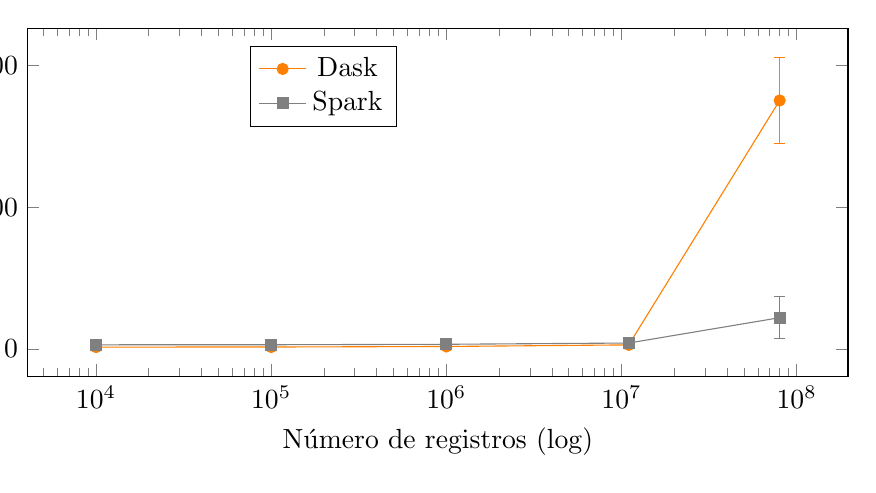
\begin{tikzpicture}[trim axis left, trim axis right]
\begin{axis}[
	xlabel = Número de registros (log),
	ylabel = Duración en segundos,
	legend style={at={(0.45,0.95)}},
	xmode=log,
	% ymode=log,
	width=12cm,
	height=6cm
	]
  \addplot+[orange,mark options={fill=orange},error bars/.cd,y dir=both,y explicit] 
    table[x=x,y=y,y error=error] {
      x   y   error
      10000 1.395 0.039
      100000 1.433 0.085
      1000000 1.817 0.039
      11000000 2.941 0.119
      80000000 175.456 30.511
    };
    
  \addplot+[gray,mark options={fill=gray},error bars/.cd,y dir=both,y explicit] 
    table[x=x,y=y,y error=error] {
      x   y   error
      10000 2.993 0.057
      100000 3.048 0.054
      1000000 3.365 0.043
      11000000 4.253 0.95
      80000000 22.14 14.685
    };
    \legend {Dask, Spark}
\end{axis}
\end{tikzpicture}
\caption{Duración promedio del proceso elimina\_nulos en diferentes muestras.}
\label{lineas:local-elimina-nulos}
\end{figure}

\subsubsection{Proceso de obtención de ruta mínima mediante el algoritmo \textit{Dijkstra}}

Este proceso tiene múltiples operaciones como conteos, filtrados, ordenamientos, etc. No obstante, su característica más importante es que se trata de un algoritmo iterativo, lo cual ayudará a evaluar cuál de los dos \textit{frameworks} es mejor en el almacenamiento temporal de resultados intermedios, en la creación de nuevos \textit{DataFrames} y en el manejo de memoria. El resultado de este algoritmo varía de acuerdo a la ruta calculada en el algoritmo, y como cada registro en el \textit{DataFrame} corresponde a un vuelo elegido este tiene entre 3 y 4 registros la mayoría de las veces, por lo que el tiempo de escritura no se considerará en este análisis.

La gráfica \ref{lineas:local-dijkstra} muestra claramente cómo la diferencia de tiempo de ejecución entre \textit{Dask} y \textit{Spark} crece junto con el tamaño de la muestra. Esto se debe a que el tiempo en cada iteración de \textit{Spark} aumenta significativamente ya que, a diferencia de \textit{Dask}, no tiene la capacidad de mantener en memoria los resultados intermedios del algoritmo y es necesario escribir a disco, lo cual es muy costoso. No obstante, es importante notar que los resultados de \textit{Dask} se convierten en un \textit{DataFrame} de \textit{Pandas} al llamar la operación \texttt{compute}, por lo que podría llegar a ser inestable si los resultados intermedios crecen demasiado.

\begin{figure}
\centering
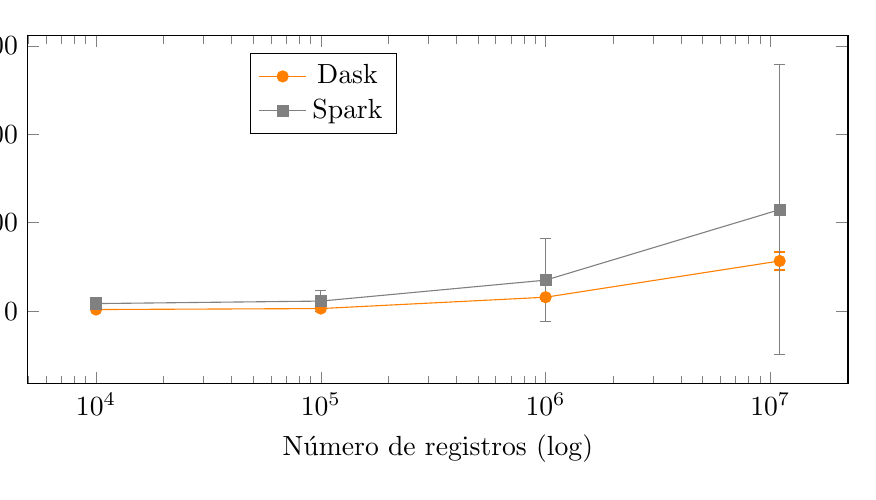
\begin{tikzpicture}[trim axis left, trim axis right]
\begin{axis}[
	xlabel = Número de registros (log),
	ylabel = Duración en segundos,
	legend style={at={(0.45,0.95)}},
	xmode=log,
	% ymode=log,
	width=12cm,
	height=6cm
	]
  \addplot+[orange,mark options={fill=orange},error bars/.cd,y dir=both,y explicit] 
    table[x=x,y=y,y error=error] {
      x   y   error
      10000 3.488 2.448
      100000 5.713 2.683
      1000000 31.371 4.527
      11000000 113.341 20.355
      % 80000000 NA NA
    };
    
  \addplot+[gray,mark options={fill=gray},error bars/.cd,y dir=both,y explicit] 
    table[x=x,y=y,y error=error] {
      x   y   error
      10000 16.957 14.158
      100000 22.62 24.204
      1000000 69.953 94.048
      11000000 229.471 327.859
      % 80000000 NA NA
    };
    \legend {Dask, Spark}
\end{axis}
\end{tikzpicture}
\caption{Duración promedio del proceso dijkstra en diferentes muestras.}
\label{lineas:local-dijkstra}
\end{figure}

\noindent ...

\newpage

\section{Ambiente en la nube}
\label{section:resultados-ambiente-nube}

\noindent ...

% Gráfica con dos colores a mano
